\documentclass[
	% -- opções da classe memoir --
	12pt,				% tamanho da fonte
	openright,			% capítulos começam em pág ímpar (insere página vazia caso preciso)
	oneside,			% twoside para impressão em verso e anverso. Oposto a oneside
	a4paper,			% tamanho do papel. 
	% -- opções da classe dc-uel --
	tccpreliminar,			% tipo do trabalho (opções: tcc, tccpreliminar, dissertacao, qualificacaoms)
					% - tcc (Versão para a Banca do TCC ou Versão Final do TCC)
					% - tccpreliminar (Versão Preliminar do TCC)
					% - dissertação (Versão para a Banca da Dissertação ou Versão Final/Revisada da Dissertação)
					% - qualificacaoms (Qualificação de Mestrado)
	]{ABNT-DC-UEL}


% ---
% PACOTES
% ---

% ---
% Pacotes fundamentais https://www.overleaf.com/project/64b9646755fec68416aede1d
% ---
\usepackage[T1]{fontenc}		% Selecao de codigos de fonte.
\usepackage[utf8]{inputenc}		% Codificacao do documento (conversão automática dos acentos)
\usepackage{graphicx}			% Inclusão de gráficos
\usepackage{pdfpages}			% Inclusão de (páginas de) arquivos PDF no documento
% ---
		
% ---
% Pacotes adicionais, usados apenas no âmbito do Modelo Canônico do abnteX2
% ---
\usepackage{lipsum}				% para geração de dummy text
% ---
\usepackage{svg}
\usepackage{amsmath}
% \usepackage[autosize]{dot2texi}
\usepackage{tikz, pgfplots}
\usepackage{listings}
\usepackage{caption}
\usepackage{subcaption}
% \usepackage[portugues, ruled, lined]{algorithm2e}
\usepackage{algorithm}
\usepackage[noend]{algpseudocode}
\usepackage{mathtools}
\usepackage{graphbox}
\usepackage{mathabx}
% \usepackage{graphviz}
\usetikzlibrary{positioning}
\usetikzlibrary{arrows.meta}
\pgfplotsset{compat=1.18}

% ---
% Informações de dados para CAPA, FOLHA DE ROSTO e outros elementos
% ---
\titulo{Aplicações do Aprendizado de Máquina na geração de código \textit{spill}}
\tituloingles{Machine Learning applications in spill code generation}
\palavraschave{Compiladores. Aprendizado de Máquina. Código spill. Alocação de registradores. Otimização}
\palavraschaveingles{Compilers. Machine Learning. Spill code. Register allocation. Optimization.}
\autor{Matheus Pires Vila Real}
\citacaoautor{VILA REAL, M.}
\data{2023}

\diadefesa{24 de novembro}
\orientador{Prof. Dr. Wesley Attrot} % É membro nato e presidente da Banca Examinadora
% \coorientador{Prof(a). Dr(a). Nome do(a) Coorientador(a)} % Pode ou não ser membro da Banca; se for, deve ser incluído como membro a seguir
\membrobancadois{Prof. Dr. Segundo Membro da Banca}
\instmembrobancadois{Universidade Estadual de Londrina}
\membrobancatres{Prof. Dr. Terceiro Membro da Banca}
\instmembrobancatres{Universidade Estadual de Londrina}

% ---
% compila o indice
% ---
\makeindex
% ---

% ----
% Início do documento
% ----
\begin{document}

% Retira espaço extra obsoleto entre as frases.
\frenchspacing 

% ----------------------------------------------------------
% ELEMENTOS PRÉ-TEXTUAIS
% ----------------------------------------------------------
% \pretextual

% ---
% Capa (elemento obrigatório)
% ---
\imprimircapa
% ---

% ---
% Folha de rosto (elemento obrigatório)
% (o * indica que haverá a ficha bibliográfica)
% ---
\imprimirfolhaderosto*
% ---


% ---
% Ficha bibliografica (elemento obrigatório para versões finais de TCC e dissertação)
% ---

% Isto é um exemplo de Ficha Catalográfica, ou ``Dados internacionais de
% catalogação-na-publicação''. Você poderá utilizar o site da biblioteca para 
% gerar esta ficha através do link: http://www.uel.br/bc/ficha/. Quando estiver
% com o documento, salve-o como PDF no diretório do seu projeto e substitua todo
% o conteúdo de implementação deste arquivo pelo comando abaixo:
%
\begin{fichacatalografica}
    \includepdf{ficha_catalografica.pdf}
\end{fichacatalografica}


% ---

% ---
% Folha de aprovação (elemento obrigatório) ==> deve ser omitida no caso de tccpreliminar
% ---

% Isto é um exemplo de Folha de aprovação, elemento obrigatório da NBR
% 14724/2011 (seção 4.2.1.3). Você pode utilizar este modelo até a aprovação
% do trabalho. Após isso, substitua todo o conteúdo deste arquivo por uma
% imagem da página assinada pela banca com o comando abaixo:
%
% \includepdf{folhadeaprovacao_final.pdf}
\imprimirfolhadeaprovacao
% ---

% ---
% Dedicatória (elemento opcional)
% ---
\begin{dedicatoria}
  \vspace*{\fill}
  \hspace{.4\textwidth}
  \begin{minipage}{.5\textwidth}
    \begin{flushright}
      \textit{Este trabalho é dedicado às crianças adultas que, quando pequenas, sonharam em se tornar cientistas.}
    \end{flushright}  
  \end{minipage}
\end{dedicatoria}
% ---

% ---
% Agradecimentos (elemento opcional, mas fortemente recomendado)
% ---
\begin{agradecimentos}
Os agradecimentos principais são direcionados à Gerald Weber, Miguel Frasson,
Leslie H. Watter, Bruno Parente Lima, Flávio de Vasconcellos Corrêa, Otavio Real
Salvador, Renato Machnievscz\footnote{Os nomes dos integrantes do primeiro
projeto abn\TeX\ foram extraídos de
\url{http://codigolivre.org.br/projects/abntex/}} e todos aqueles que
contribuíram para que a produção de trabalhos acadêmicos conforme
as normas ABNT com \LaTeX\ fosse possível.

Agradecimentos especiais são direcionados ao Centro de Pesquisa em Arquitetura
da Informação\footnote{\url{http://www.cpai.unb.br/}} da Universidade de
Brasília (CPAI), ao grupo de usuários
\emph{latex-br}\footnote{\url{http://groups.google.com/group/latex-br}} e aos
novos voluntários do grupo
\emph{\abnTeX}\footnote{\url{http://groups.google.com/group/abntex2} e
\url{http://abntex2.googlecode.com/}}~que contribuíram e que ainda
contribuirão para a evolução do \abnTeX.

\end{agradecimentos}
% ---

% ---
% Epígrafe (elemento opcional)
% ---
\begin{epigrafe}
  \vspace*{\fill}
  \hspace{.4\textwidth}
  \begin{minipage}{.5\textwidth}   
    \begin{flushright}
	\textit{
    ``Não vos amoldeis às estruturas deste mundo,
      mas transformai-vos pela renovação da mente,
      a fim de distinguir qual é a vontade de Deus:
      o que é bom, o que Lhe é agradável, o que é perfeito.\\
      (Bíblia Sagrada, Romanos 12, 2))}
    \end{flushright}
  \end{minipage}
\end{epigrafe}
% ---

% ---
% RESUMOS
% ---

% ---
% Resumo em Português (elemento obrigatório)
% ---
\begin{resumo}
A alocação de registradores é uma das otimizações de código mais significativas do processo de compilação de um programa. Mas, devido à natureza dos algoritmos empregados nas implementações tradicionais, ela caracteriza-se como um prolema NP-completo, o qual é difícil de se resolver de maneira ótima. Nesse contexto, ao longo dos anos foram sendo propostas heurísticas e ajustes visando tornar as técnicas de geração de código \textit{spill} mais precisas e menos custosas. Com o crescimento da relevância do aprendizado de máquina (\textit{machine learning}) --- área da inteligência artificial, que engloba o desenvolvimento de modelos complexos de categorização e predição treinados de maneira algorítmica --- surge a perspectiva de integração de ambas as áreas. Isto posto, este trabalho se propõe a vislumbrar o estado da arte da aplicação do aprendizado de máquina na alocação de registradores e investigar as possibilidades práticas de implementação de alocadores utilizando modelos treinados por \textit{machine learning}.
\end{resumo}
% ---

% ---
% Resumo em Inglês (elemento obrigatório)
% ---
% O ambiente Abstract (com A maiúsculo) é definido no estilo dc-uel
\begin{Abstract}
Register allocation is highlighted as one of the key code optimizations throughout a program's compilation process. It is, however, a NP-complete problem, due to the nature of the traditional implementations, which are unable to obtain optimal solutions in reasonable time. In this context, several heuristics and adjustments have been proposed over the course of the years in order to improve the precision and the speed of register allocators. Machine learning, in the other hand, is a field of artificial intelligence encompassing the development of complex classification and prediction models which are trained in an algorithmic way, that grew in relevance and became widely researched recently. Therefore, efforts to apply machine learning techniques to register allocation, aiming to improve spill code generation, arose. This work is intended to examine the current state-of-the-art of the integration of both fields and investigate the implementation possiblities of register allocators that widely employ machine learning models in their inner workings.
\end{Abstract}
% ---

% ---
% Lista de ilustrações (elemento opcional, mas fortemente recomendado)
% ---
\pdfbookmark[0]{\listfigurename}{lof}
\listoffigures*
\cleardoublepage
% ---

% ---
% Lista de tabelas (elemento opcional, mas fortemente recomendado)
% ---
\pdfbookmark[0]{\listtablename}{lot}
\listoftables*
\cleardoublepage
% ---

% ---
% Lista de abreviaturas e siglas (elemento opcional)
% ---
\begin{siglas}
  % \item[ABNT] Associação Brasileira de Normas Técnicas
  % \item[BNDES] Banco Nacional de Desenvolvimento Econômico e Social
  % \item[IBGE] Instituto Nacional de Geografia e Estatística
  % \item[IBICT] Instituto Brasileiro de Informação em Ciência e Tecnologia
  % \item[NBR] Norma Brasileira
  \item[CPU] \textit{Central Processing Unit}
\end{siglas}
% ---

% ---
% Lista de símbolos (elemento opcional)
% ---
% \begin{simbolos}
%   \item[$ \Gamma $] Letra grega Gama
%   \item[$ \Lambda $] Lambda
%   \item[$ \zeta $] Letra grega minúscula zeta
%   \item[$ \in $] Pertence
% \end{simbolos}
% ---

% ---
% Sumario (elemento obrigatório)
% ---
\pdfbookmark[0]{\contentsname}{toc}
\tableofcontents*
\cleardoublepage
% ---



% ----------------------------------------------------------
% ELEMENTOS TEXTUAIS
% ----------------------------------------------------------
\textual
\pagestyle{dc-uel-header} % Configura cabeçalho para apresentar apenas números de página


% ----------------------------------------------------------
% Introdução
% ----------------------------------------------------------
\chapter{Introdução}
Os compiladores constituem uma das classes de programa mais importantes na Ciência da Computação, cuja principal função é a tradução de código-fonte de uma linguagem de programação para outra. Usualmente, esse processo é empregado para transformar código de alto nível em linguagem de máquina de baixo nível, executável diretamente pelo processador de determinada arquitetura-alvo. \cite{aho:07}.

Para atingir esse objetivo, o compilador deve submeter o programa original a uma série de análises --- léxica, sintática e semântica --- a fim de criar uma representação lógica de sua estrutura e prosseguir com a geração de código. Entre essas duas etapas, é desejável efetuar algumas otimizações a fim de tornar o binário final mais eficiente do ponto de vista de execução e mais coerente com as especificidades da arquitetura-alvo \cite{muchnick:97}.

Dentre as etapas de otimização, destaca-se a alocação de registradores, onde o compilador deve distribuir os registradores para as variáveis utilizadas ao longo do fluxo de execução do programa. Os registradores são componentes microarquiteturais diretamente disponíveis ao processador, e caracterizam-se como as unidades de memória de mais rápido acesso \cite{mittal:16}. Contudo, sendo eles um recurso finito, surge a possibilidade de não haverem registradores o suficiente para comportar todos os valores e resultados intermediários em memória de uma única vez \cite{aho:07}.

Nesses casos, há a necessidade de se mapear algumas variáveis para a memória principal, e o compilador deve então introduzir no código instruções de acesso à memória para salvar e recuperar os valores lá armazenados. Essas instruções são denominadas código \textit{spill}, ou \textit{spill code} \cite{briggs:92}. Um esquema de alocação ideal deve buscar minimizar o tráfego entre a memória principal e a CPU, visto que essas operações, em comparação com o acesso a registradores, são significativamente mais lentas e dispendiosas do ponto de vista energético. As operações em memória representam de 50\% a 75\% dos gastos de energia de um sistema computacional \cite{verma:06}, e um alocador sofisticado pode proporcionar uma melhora de até 250\% no tempo de execução de um programa comparado a um alocador simples \cite{pereira:08}.

A abordagem tradicional emprega a coloração de grafo como abstração para representar o processo de atribuição dos registradores físicos para as variáveis virtuais. Nesse modelo, os valores em memória --- chamados de registradores virtuais da representação intermediária do código --- são expressos como os nós de um grafo a ser colorido; as arestas representam as relações de interferência entre os registradores virtuais, isto é, a presença de intersecções entre o tempo de vida dos valores em memória, enquanto que a coloração em si seria o processo de encontrar registradores físicos disponíveis para cada variável \cite{chaitin:81}.

Contudo, produzir uma alocação eficiente não é uma tarefa trivial. A coloração de grafos é um problema NP-completo, isto é, não há algoritmos determinísticos que a resolvam em tempo polinomial \cite{karp:72}, e descobrir a mera quantidade de cores necessárias para colorir um grafo é um problema difícil \cite{garey:76}. Ademais, uma implementação ingênua pode introduzir \textit{spill code} desnecessário ao longo de todo o tempo de vida de um registrador virtual \cite{bergner:97}, ou realizar escolhas ruins sobre quais variáveis enviar para a memória principal, ao eleger valores frequentemente utilizados no código e que exigirão uma grande quantidade de acessos ou escritas à memória \cite{bernstein:89}.

Ao longo dos anos, soluções para se contornar as dificuldades em se gerar código \textit{spill} de maneira eficiente foram propostas: ajustes no algoritmo original, visando tornar a introdução de instruções \texttt{load}/\texttt{store} mais precisa nos pontos de interferência necessários \cite{chaitin:82, briggs:92, briggs2:92, cooper:98}, e a utilização de heurísticas para cálculo de custo de \textit{spill}, visando melhorar a qualidade das escolhas de quais variáveis mapear para a memória principal. Infelizmente, as heurísticas dependem de uma boa quantidade de ajustes para propiciar um desempenho adequado. O desenvolvimento de um conjunto de heurísticas para uma arquitetura-alvo específica ainda é feito através de tentativa e erro, e o ajuste fino das funções prioritárias é um processo tedioso \cite{amarasinghe:03}.

O aprendizado de máquina (\textit{machine learning}), por sua vez, é uma área da inteligência artificial que abrange o desenvolvimento de modelos e agentes inteligentes treinados de maneira algorítmica. Eles realizam tarefas de predição e classificação probabilísticas a partir de parâmetros de entrada, e são calibrados após sucessivas iterações de treinamento, onde os resultados de saída são confrontados com um conjunto de dados previamente conhecidos sobre o problema, de modo a se calcular um erro e ajustar os parâmetros internos do modelo para minimizá-lo \cite{sharma:21}.

Nas últimas décadas, o aprendizado de máquina e a inteligência artificial como um todo vem avançando consideravelmente, graças ao crescimento do poder computacional das máquinas e conforme cada vez mais dados são gerados e coletados \cite{alpaydin:20}. Esse cenário expande os horizontes para a integração de ambas as áreas, que almeja o desenvolvimento de melhores heurísticas e métodos para otimizar a alocação de registradores empregando técnicas de aprendizado de máquina. Trabalhos vêm sendo publicados explorando a interdisciplinaridade de ambas as áreas e trazendo resultados animadores ou, ao menos, de interesse, como é o caso das pesquisas de Amarasinghe \textit{et al.}, Das \textit{et al.} e VenkataKeerthy \textit{et al.} \cite{amarasinghe:03, das:20, venkatakeerthy:23}.

Este trabalho se propõe a investigar a aplicação das técnicas de aprendizado de máquina na alocação de registradores, particularmente sua utilidade na geração de código \textit{spill}. Ele irá contemplar o estado da arte da alocação de registradores e, apoiado no conhecimento acadêmico sobre a área, serão propostos métodos de alocação e heurísticas que utilizam \textit{machine learning}. Utilizando as ferramentas disponíveis na infraestrutura LLVM --- um \textit{framework} utilizado na implementação de compiladores de produção, é esperado desenvolver um modelo de aprendizado que auxilie nas etapas da alocação tradicional, e que tenha um desempenho ao menos comparável ao dos alocadores do \textit{framework}.

% Explicar seções

% ----------------------------------------------------------
% PARTE
% ----------------------------------------------------------
% A organização dos capítulos em partes só é recomendada caso o texto seja muito extenso
% Não é comum dividir o trabalho em partes em TCCs e dissertações de mestrado

%\part{Preparação da pesquisa}

% ----------------------------------------------------------
% Capitulo com exemplos de comandos inseridos de arquivo externo 
% ----------------------------------------------------------

% \include{abntex2-modelo-include-comandos}

\chapter{Alocação de Registradores}

A alocação de registradores é uma etapa de otimização responsável por assinalar registradores físicos às variáveis presentes na representação intermediária (\textit{IR}) produzida pelo \textit{front-end} do compilador. A \textit{IR} é produzida após a conclusão das análises léxica, sintática e semântica no código-fonte --- onde o compilador extrai as informações sobre o fluxo de execução e operações aritméticas --- e consiste, usualmente, numa simplificação com menos abstrações do programa inicial, chamada código de três endereços \cite{aho:07}.

Essa simplificação representa o programa como uma sequência de instruções de até três operandos, compostas por expressões de atribuição com operações binárias ou desvios. Para fins de análise, o código é organizado em um grafo onde cada nó contém uma quantidade de instruções, chamado grafo de controle de fluxo (\textit{control flow graph}, ou CFG). Ele denota a sequência de execução do programa e permite ao compilador realizar as análises necessárias para se efetuar otimizações no código, chamadas de \textit{control flow analysis} \cite{allen:70}.

A figura \ref{fig:1} é um exemplo de um trecho de código qualquer, em linguagem C, que apresenta operações aritméticas e uma estrutura de controle. Após a análise dos elementos do código-fonte, o modelo abstrato obtido é similar à árvore da figura \ref{fig:2a}. A partir desse modelo, é produzida a representação intermediária equivalente, mostrada na figura \ref{fig:2b}.

\begin{figure}[ht]
    \centering
    
    \begin{lstlisting}[language=c, frame=single]
        do {
            j = a + a * (c * d - d);
            i--;
        } while (i > 0);
        i = j;
    \end{lstlisting}
    \caption{Exemplo de código C apresentando expressões aritméticas e estruturas de controle.}
    \label{fig:1}
\end{figure}

\begin{figure}
    \begin{subfigure}{0.6\textwidth}
        \centering
        
        \begin{tikzpicture} [level 1/.style={sibling distance=40mm},level 2/.style={sibling distance=20mm},
                        level 3/.style={sibling distance=15mm}]
            \node {programa}
            child {node {do..while}
              child {node {>}
                child {node {i}}
                child {node {0}}
              }
              child {node {=}
                child {node {j}}
                child {node {+}
                    child {node {a}}
                    child {node {*}
                        child {node {a}}
                        child {node {-}
                            child {node {*}
                                child {node {c}}
                                child {node {d}}
                            }
                            child {node {d}}
                        }
                    }
                }
              }
              child {node {- -} child {node {i}}}
            }
            child {node {=}
                child {node {i}}
                child {node {j}}
            };
        \end{tikzpicture}
        \caption{Árvore sintática abstrata representando o código da figura 1.}
        \label{fig:2a}
    \end{subfigure}
    \begin{subfigure}{0.3\textwidth}
        \centering
        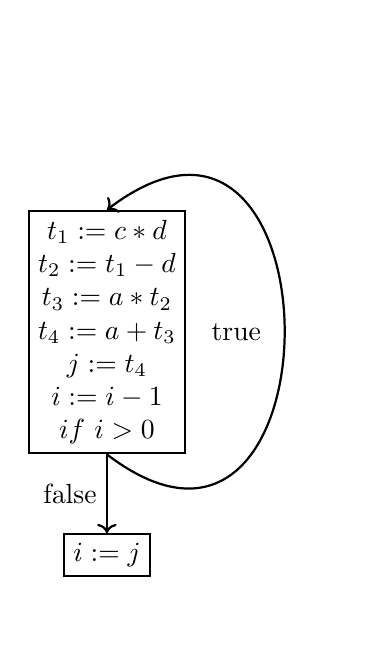
\begin{tikzpicture}[
        CFG/.style={rectangle, draw=black!100, fill=white!100, thick, minimum size=5mm, align=center},
        ]
            \node[CFG] (B0) {$t_1:=c*d$\\
                             $t_2:=t_1-d$\\
                             $t_3:=a*t_2$\\
                             $t_4:=a+t_3$\\
                             $j:=t_4$\\
                             $i:=i-1$\\
                             $if$ $i>0$};
            \node[CFG] (B1) [below=of B0] {$i:=j$};
            \node[right = 0.2cm of B0] {true};
            \coordinate[above right = 2.3cm and 2cm of B0] (a) {};
            \coordinate[below right = 2.3cm and 2cm of B0] (b) {};
    
            \draw[->, thick] (B0.south) to node[left] {false} (B1.north);
            \draw[->, thick] (B0.south) .. controls (b) and (a)  .. (B0.north);
        \end{tikzpicture}
        \caption{Grafo de controle de fluxo equivalente.}
        \label{fig:2b}
    \end{subfigure}
    \label{fig:2}
\end{figure}

Devido à natureza do código de três endereços, os valores intermediários computados no cálculo de expressões aritméticas complexas e avaliação de estruturas de controle são expostos na forma de variáveis temporárias, que se juntam às variáveis definidas pelo programador para formar o conjunto dos valores em memória utilizados pelo programa. Esses valores são denominados registradores virtuais, e é trabalho do alocador decidir onde eles serão armazenados \cite{muchnick:97}.

Os registradores virtuais são endereços simbólicos que serão traduzidos em endereços reais após o processo de alocação de registradores. Eles são gerados de maneira incremental pelo compilador de modo a substituir os endereços reais, para possibilitar uma representação abstrata do programa na forma de código de três endereços e permitir a realização de inúmeras otimizações, sem que a disposição dos endereços de memória seja um entrave para a manipulação da IR \cite{muchnick:97}.

\section{\textit{Liveness Analysis} e Interferências}

Em posse de uma representação intermediária contendo registradores virtuais, o compilador prossegue para a tarefa de mapeá-los para endereços de memória ou registradores físicos. Essa tarefa impõe alguns grandes obstáculos: o número de registradores disponíveis é limitado e em alguns casos bem pequeno, além do fato de que dois valores de memória não podem ocupar um único registrador físico ao mesmo tempo.

Sendo assim, para corretamente alocar os recursos de memória da CPU de modo a comportar as variáveis utilizadas pelo programa, o compilador deve computar os pontos de utilização dos valores ao longo do programa e determinar quando uma variável está viva ou não. Esse processo é denominado análise de longevidade, ou \textit{liveness analysis}, e é uma variação da análise de fluxo de dados também efetuada em outras otimizações. 

Uma variável é dita viva no ponto que antecede diretamente a execução de uma instrução se ela contém um valor que será utilizado futuramente, ou, em outra palavras, se ela será lida antes da próxima redefinição de seu valor. O conjunto de todos os pontos pelos quais uma variável contendo um valor está viva é chamado de \textit{live range}. Entretanto, uma única variável pode ser quebrada em vários \textit{live ranges}, conforme o valor que ela armazena não será mais utilizado ou é redefinido, dando origem a objetos alocáveis distintos \cite{aho:07}.

Quando dois \textit{live ranges} $v_i$ e $v_j$ se sobrepõe em determinado ponto, diz-se que há uma interferência entre eles. Em outras palavras, eles interferem pois a intersecção entre seus conjuntos de pontos não é vazia. Isso significa que ambos os valores presentes em $v_i$ e $v_j$ não podem ser mapeados para o mesmo registrador físico, pois ambos devem ser mantidos em memória integralmente para algum uso posterior. A figura \ref{fig:3} mostra dois blocos básicos com variáveis e seus respectivos \textit{live ranges}. Nesse exemplo, a variável $a$ interfere com $b$ e $c$.

Se dois \textit{live ranges} $v_i$ e $v_j$ estiverem conectados por uma instrução de cópia na forma $v_i := v_j$ e não interferirem entre si, os dois valores podem ser armazenados no mesmo registrador. Esse ato é denominado coalescimento, ou \textit{coalescing}, e pode promover um ganho significativo na qualidade do código gerado ao eliminar instruções de cópia desnecessárias \cite{appel:96, chaitin:82, briggs:92}.

% EXEMPLOS.
\begin{figure}
    \centering
    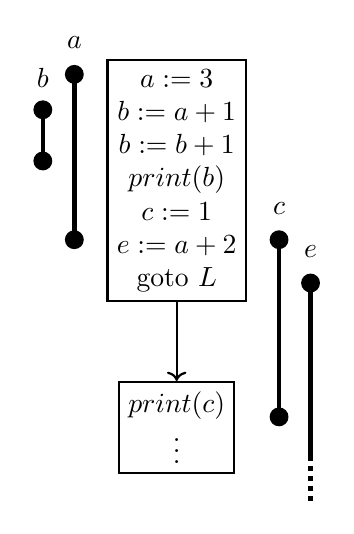
\begin{tikzpicture}[
    CFG/.style={rectangle, draw=black!100, fill=white!100, thick, minimum size=5mm, align=center},
    ]
        \node[CFG] (B0) {$a:=3$\\
                         $b:=a+1$\\
                         $b:=b+1$\\
                         $print(b)$\\
                         $c:=1$\\
                         $e:=a+2$\\
                         goto $L$};
        \node[CFG] (B1) [below=of B0] {$print(c)$\\$\vdots$};
        \draw[->, thick] (B0.south) -- (B1.north);
        
        \draw[black, ultra thick] (-1.3, -0.75) -- (-1.3, 1.35);
        \filldraw[black, thick] (-1.3, -0.75) circle (3pt);
        \filldraw[black, thick] (-1.3, 1.35) circle (3pt);
        \node at (-1.3, 1.75) {$a$};
        
        \draw[black, ultra thick] (-1.7, 0.25) -- (-1.7, 0.90);
        \filldraw[black, thick] (-1.7, 0.25) circle (3pt);
        \filldraw[black, thick] (-1.7, 0.90) circle (3pt);
        \node at (-1.7, 1.30) {$b$};

        \draw[black, ultra thick] (1.3, -0.75) -- (1.3, -3);
        \filldraw[black, thick] (1.3, -0.75) circle (3pt);
        \filldraw[black, thick] (1.3, -3) circle (3pt);
        \node at (1.3, -0.35) {$c$};

        \draw[black, ultra thick] (1.7, -1.3) -- (1.7, -3.5);
        \filldraw[black, thick] (1.7, -1.3) circle (3pt);
        \draw[black, ultra thick, dotted] (1.7, -3.5) -- (1.7, -4.10);
        \node at (1.7, -0.9) {$e$};
    \end{tikzpicture}
    \caption{Dois blocos básicos contendo as variáveis $a$, $b$, $c$ e $e$, com seus respectivos \textit{live ranges} indicados.}
    \label{fig:3}
\end{figure}

\section{Geração de Código \textit{Spill}}

O número de registradores físicos necessários para comportar os \textit{live ranges} em um ponto do código é uma métrica conhecida como pressão de registradores. Quando esse número excede a quantidade de registradores disponíveis para a alocação, faz-se necessário armazenar algum \textit{live range} na memória principal. Para isso, são introduzidas as instruções de acesso a memória \texttt{store}, para escrever, e \texttt{load} para recuperar um valor em memória. Essas instruções são denominadas código \textit{spill}, e tem por efeito fragmentar o \textit{live range} escolhido ao redor do ponto de grande pressão, a fim de reduzi-la \cite{chaitin:81}. Ao longo do curso de execução de um programa, uma mesma variável pode ser ser armazenada em registradores e posteriormente ser enviada para a memória, e ter seu \textit{live range} particionado \cite{eisl:16}.

% Exemplos
\begin{figure}
    \centering
    \begin{subfigure}{0.4\textwidth}
        \centering
        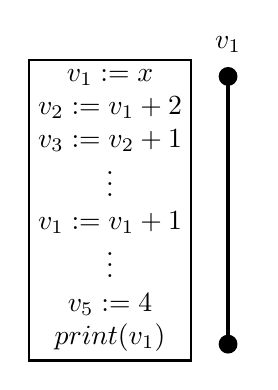
\begin{tikzpicture}[
        CFG/.style={rectangle, draw=black!100, fill=white!100, thick, minimum size=5mm, align=center},
        ]
            \node[CFG] (B0) {$v_1:=x$\\
                             $v_2:=v_1+2$\\
                             $v_3:=v_2+1$\\
                             $\vdots$\\
                             $v_1:=v_1+1$\\
                             $\vdots$\\
                             $v_5:=4$\\
                             $print(v_1)$};
            
            \draw[black, ultra thick] (1.5, -1.70) -- (1.5, 1.70);
            \filldraw[black, thick] (1.5, -1.70) circle (3pt);
            \filldraw[black, thick] (1.5, 1.70) circle (3pt);
            \node at (1.5, 2.10) {$v_1$};
        \end{tikzpicture}
        \caption{Teste}
    \end{subfigure}
    \begin{subfigure}{0.4\textwidth}
        \centering
        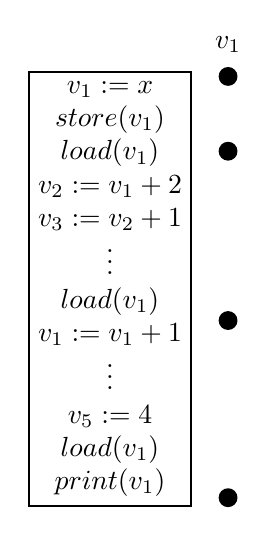
\begin{tikzpicture}[
        CFG/.style={rectangle, draw=black!100, fill=white!100, thick, minimum size=5mm, align=center},
        ]
            \node[CFG] (B0) {$v_1:=x$\\
                             $store(v_1)$\\
                             $load(v_1)$\\
                             $v_2:=v_1+2$\\
                             $v_3:=v_2+1$\\
                             $\vdots$\\
                             $load(v_1)$\\
                             $v_1:=v_1+1$\\
                             $\vdots$\\
                             $v_5:=4$\\
                             $load(v_1)$\\
                             $print(v_1)$};
            
            % \draw[black, ultra thick] (1.5, 2.70) -- (1.5, -1.70);
            \node at (1.5, 3.1) {$v_1$};
            \filldraw[black, thick] (1.5, 2.70) circle (3pt);
            \filldraw[black, thick] (1.5, 1.75) circle (3pt);
            \filldraw[black, thick] (1.5, -0.4) circle (3pt);
            \filldraw[black, thick] (1.5, -2.65) circle (3pt);
        \end{tikzpicture}
        \caption{Teste}
    \end{subfigure}
    \caption{Dois blocos básicos contendo as variáveis $a$, $b$, $c$ e $e$, com seus respectivos \textit{live ranges} indicados.}
    \label{fig:4}
\end{figure}

Esse artifício, no entanto, produz um código mais lento. As instruções de acesso à memória consomem significativamente mais ciclos do que operações aritméticas simples em registradores e desvios. A inserção de \textit{spill code} em locais inapropriados, como em laços de repetição ou trechos que serão frequentemente executados, podem causar um grande \textit{overhead} que derruba a performance do executável gerado. Um alocador eficiente tem a tarefa de minimizar a quantidade de acessos à memória gerados o quanto for possível, e ser preciso em suas escolhas sobre quais variáveis selecionar para \textit{spill} e a colocação das instruções.

\section{Alocação via Coloração de Grafos}

A alocação de registradores por coloração de grafos é a abordagem dominante para o desenvolvimento de alocadores na atualidade. Ela foi implementada pela primeira vez por Chaitin \textit{et al.} em 1980, em um compilador experimental da linguagem PL/I para o IBM System/370 \cite{chaitin:81}, e foi o primeiro método amplamente aplicado para alocação global de registradores, onde os registradores são alocados para toda a unidade de compilação (função) de uma só vez, em vez de alocá-los por bloco \cite{eisl:16}.

Seja $G = (V, E)$ um grafo não-direcionado, onde os vértices $v \in V$ representam os \textit{live ranges} e as arestas $e \in E$, as interferências, tal que $e_n = (v_i, v_j)$ simboliza a existência de uma interferência entre $v_i$ e $v_j$. O grafo $G$ é dito $k$-colorível se houver uma função $cor: V \to \{1,...,k\}$ tal que $cor(v_i) \ne cor(v_j)$, para todo $v_i$ e $v_j$ em que existir uma aresta
$e_n = (v_i, v_j)$. A alocação é reduzida, então, a encontrar o mapeamento dado pela função $cor$, onde $k$ é o número de registradores físicos presentes na arquitetura-alvo.

\begin{figure}[ht]
    \centering
    \includesvg[scale=0.7]{img/peterson-graph.svg}
    \caption{Grafo de Peterson, colorido com 3 cores.}
    \label{fig:5}
\end{figure}

Entretanto, computar uma solução ótima não é trivial. A coloração de grafo é um clássico problema NP-completo \cite{karp:72} --- determinar a $k$-colorabilidade de um grafo possui complexidade exponencial e logo torna-se inviável para casos que envolvem muitos registradores virtuais \cite{lawler:76, bjorklund:09}, e a mera tarefa de determinar o número mínimo de cores para se colorir um grafo é um problema NP-\textit{hard} \cite{garey:76}.

\subsection{Alocador de \textit{Chaitin}}

Chaitin \textit{et al.} \cite{chaitin:82} formalizaram, em 1982, seu algoritmo de alocação global de registradores via coloração de grafo. A figura \ref{fig:7} esquematiza a execução do procedimento, que consiste em construir um grafo de interferência e manipulá-lo em etapas que estão descritas a seguir:

\begin{enumerate}
    \item \textit{Renumber} --- encontrar todos os \textit{live ranges} dentro do escopo da função ou procedimento, e lhes atribuir um identificador único;
    \item \textit{Build} --- construir o grafo de interferência $G = (V,E)$, onde cada \textit{live range} se torna um vértice $v\in 
    V$ e as arestas $(v_i,v_j)\in E$ são adicionadas conforme o código é varrido de maneira retrógrada e as interferências são descobertas;
    \item \textit{Coalesce} --- combinar os \textit{live ranges} que são conectados por uma única instrução de cópia $v_i:=v_j$ e não interferem entre si, de modo que os vértices correspondentes no grafo sejam combinados em um único vértice $v_{ij}$. A instrução de cópia pode ser removida da IR, e as etapas de \textit{build} e \textit{coalesce} devem ser refeitas devido à modificação no código;
    \item \textit{Spill cost} --- computar o custo de \textit{spill} para cada \textit{live range}. Esse custo é uma estimativa do aumento no tempo de execução se um dado vértice for mapeado para a memória principal, aumento esse que é proporcional ao número de vezes que as instruções de \texttt{store} e \texttt{load} inseridas serão executadas;
    \item \textit{Simplify} --- remover os vértices tal que $grau(v)<k$, onde $grau(v)$ é o número de arestas de $v$ e $k$ é número de cores. Isso pode ser feito pois, se um vértice possui um número de arestas menor do que o número de cores, ele certamente é colorível. Sendo assim, após a remoção, o vértice deve ser adicionado a uma pilha auxiliar $S$, que serve como estrutura de controle da ordem de remoção.
    
    Se não houverem vértices aptos a serem removidos, algum deve ser escolhido para sofrer \textit{spill}. A prioridade de \textit{spill} é calculada utilizando o custo calculado na etapa anterior, sendo igual a $custo(v)/grau(v)$. O vértice que apresentar o menor custo então é escolhido e a etapa \textit{spill code} é acionada; 
    \item \textit{Spill code} --- o código é alterado com a inserção de instruções de acesso à memória, e o algoritmo deve reiniciar a partir da etapa \textit{renumber};
    \item \textit{Select} --- assinalar cores aos vértices de $G$, os desempilhando de $S$ um a um, na ordem reversa à que foram removidos na etapa anterior. Se a geração de \textit{spill code} não foi acionada, seguramente todos os vértices receberão uma cor tal que $cor(v_i)\ne cor(v_j)$ onde $v_i$ e $v_j$ são vizinhos.
\end{enumerate}

\begin{figure}
    \centering
    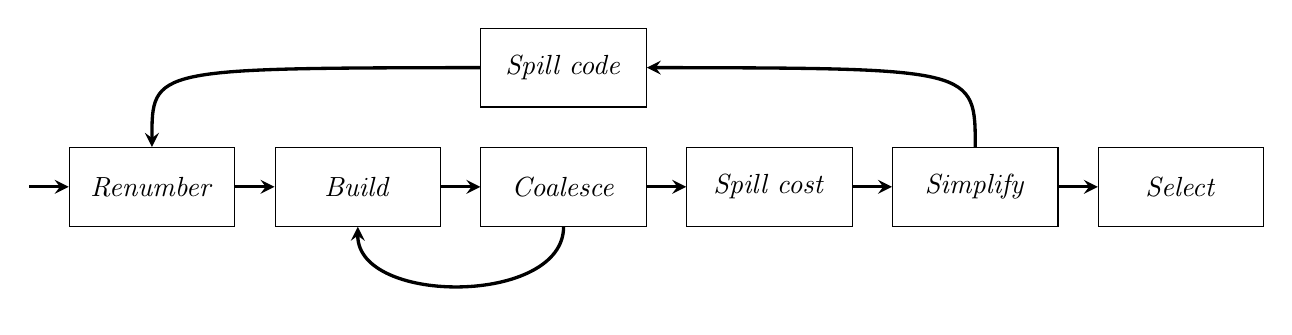
\begin{tikzpicture}[
        node distance= 1cm and 0.5cm,
        box/.style={draw, rectangle, minimum width=2.1cm, minimum height=1cm, align=center},
        arrow/.style={very thick, ->, >=stealth},
    ]
        \node[box] (renumber) {\textit{Renumber}};
        \node[box, right = of renumber] (build) {\textit{Build}};
        \node[box, right = of build] (coalesce) {\textit{Coalesce}};
        \node[box, right = of coalesce] (cost) {\textit{Spill cost}};
        \node[box, right = of cost] (simplify) {\textit{Simplify}};
        \node[box, right = of simplify] (select) {\textit{Select}};
        \node[box, above = 0.5cm of coalesce] (spill) {\textit{Spill code}};
        \coordinate[above = of simplify] (bezier1);
        \coordinate[above = of renumber] (bezier2);
        \coordinate[below = of coalesce] (bezier3);
        \coordinate[below = of build] (bezier4);
        \coordinate[left = of renumber] (start);

        \draw[arrow] (renumber) -- (build);
        \draw[arrow] (build) -- (coalesce);
        \draw[arrow] (coalesce) -- (cost);
        \draw[arrow] (cost) -- (simplify);
        \draw[arrow] (simplify) -- (select);

        \draw[arrow] (simplify.north) .. controls (bezier1) .. (spill.east);
        \draw[arrow] (spill.west) .. controls (bezier2) .. (renumber.north);
        \draw[arrow] (coalesce.south) .. controls (bezier3) and (bezier4) .. (build.south);
        \draw[arrow] (start) -- (renumber.west);
    \end{tikzpicture}
    \caption{Esquema do algoritmo de Chaitin.}
    \label{fig:6}
\end{figure}

\subsection{Alocador de \textit{Chaitin-Briggs}}

Briggs \cite{briggs:92} propôs uma série de alterações ao algoritmo de Chaitin a fim de corrigir uma série de defeitos que sua versão inicial apresentava. Notavelmente, ele sugeriu um atraso na etapa de geração de \textit{spill code} para produzir alocações mais eficientes e alguns ajustes no processo de coalescimento do alocador, a fim de otimizar o tratamento de instruções de cópia.

Em um trabalho anterior, de 1989 \cite{briggs:89}, Briggs \textit{et al.} demonstraram que o alocador de Chaitin era ineficiente na sua etapa de \textit{simplify}, ao gerar \textit{spill} em grafos que são trivialmente coloríveis. Um exemplo empregado pelo próprio Briggs é o de um grafo em forma de losango, com quatro vértices com duas arestas cada, mostrado na figura \ref{fig:8}. Esse grafo é visivelmente colorível para um número de cores $k=2$; no entanto, o alocador de Chaitin iria fatalmente enviar algum registrador virtual para a memória pois, na etapa de \textit{simplify}, não haveriam vértices onde $grau(v)<2$, e algum deles seria imediatamente enviado para \textit{spill}.

A solução proposta por Briggs foi o \textit{optimistic coloring} --- nessa abordagem, a etapa de geração de código \textit{spill} é adiada para depois da etapa de \textit{select}. Se por acaso, durante o \textit{simplify}, não houverem vértices tal que $grau(v)<k$, deve ser escolhido um candidato a \textit{spill} $s$ que será removido do grafo, permitindo continuar com a simplificação. Prosseguindo para o \textit{select}, se não for possível assinalar uma cor para $s$ quando este for desempilhado, somente então a etapa de geração de \textit{spill code} é acionada e $s$ é enviado para a memória. Dessa maneira, grafos $k$-coloríveis que travariam o alocador de Chaitin com $k$ cores tornam-se solúveis.

\begin{figure}
    \centering
    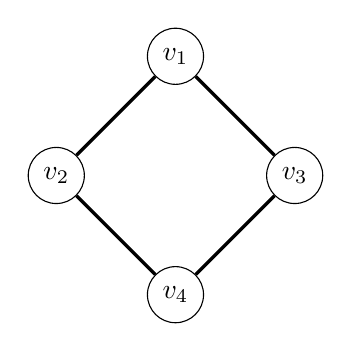
\begin{tikzpicture}[
        node/.style={draw,circle}
    ]
    \node[node] (v_1) {$v_1$};
    \node[node, below left = of v_1] (v_2) {$v_2$};
    \node[node, below right = of v_1] (v_3) {$v_3$};
    \node[node, below left = of v_3] (v_4) {$v_4$};

    \draw[-, very thick] (v_1) -- (v_2);
    \draw[-, very thick] (v_2) -- (v_4);
    \draw[-, very thick] (v_3) -- (v_4);
    \draw[-, very thick] (v_3) -- (v_1);
        
    \end{tikzpicture}
    \caption{Grafo $2$-colorível que seria incorretamente colorido pelo alocador de Chaitin.}
    \label{fig:7}
\end{figure}

Além disso, o algoritmo de Chaitin, na etapa de \textit{coalesce}, poderia transformar um grafo $k$-colorível em um não-colorível ao combinar dois vértices $v_i$ e $v_j$ em um único vértice $v_{ij}$, onde $grau(v_{ij})\geq k$. Dessa forma, Briggs \textit{et al.} \cite{briggs2:92} propuseram o \textit{conservative coalescing}, que consiste em somente coalescer dois vértices se a união de ambos tiver um grau menor do que o número de cores, sendo assim garantidamente colorível.

\begin{figure}
    \centering
    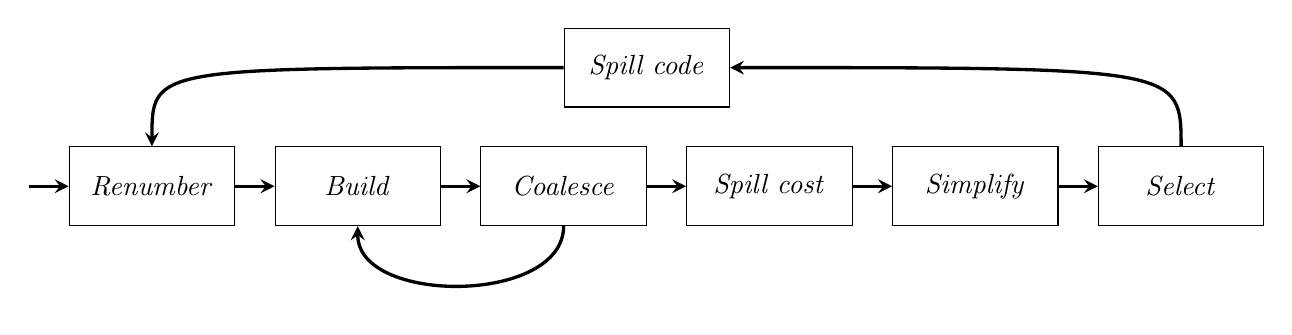
\begin{tikzpicture}[
        node distance= 1cm and 0.5cm,
        box/.style={draw, rectangle, minimum width=2.1cm, minimum height=1cm, align=center},
        arrow/.style={very thick, ->, >=stealth},
    ]
        \node[box] (renumber) {\textit{Renumber}};
        \node[box, right = of renumber] (build) {\textit{Build}};
        \node[box, right = of build] (coalesce) {\textit{Coalesce}};
        \node[box, right = of coalesce] (cost) {\textit{Spill cost}};
        \node[box, right = of cost] (simplify) {\textit{Simplify}};
        \node[box, right = of simplify] (select) {\textit{Select}};
        \coordinate[above = of select] (bezier1);
        \coordinate[above = of renumber] (bezier2);
        \coordinate[below = of coalesce] (bezier3);
        \coordinate[below = of build] (bezier4);
        \coordinate[left = of renumber] (start);
        \coordinate[above = of cost] (d);
        \node[box, left = of d] (spill) {\textit{Spill code}};

        \draw[arrow] (renumber) -- (build);
        \draw[arrow] (build) -- (coalesce);
        \draw[arrow] (coalesce) -- (cost);
        \draw[arrow] (cost) -- (simplify);
        \draw[arrow] (simplify) -- (select);

        \draw[arrow] (select.north) .. controls (bezier1) .. (spill.east);
        \draw[arrow] (spill.west) .. controls (bezier2) .. (renumber.north);
        \draw[arrow] (coalesce.south) .. controls (bezier3) and (bezier4) .. (build.south);
        \draw[arrow] (start) -- (renumber.west);
    \end{tikzpicture}
    \caption{Esquema do algoritmo de Briggs, com a etapa de geração de \textit{spill code} adiada.}
    \label{fig:8}
\end{figure}

\subsection{\textit{Outras contribuições}}

Em 1996, George e Appel \cite{appel:96} propuseram uma maneira diferente de coalescer os registradores virtuais: o \textit{iterated register coalescing} é um método mais agressivo de combinar vértices no grafo de interferência, sem adicionar novos \textit{spills} desnecessariamente. Ele consistia em executar as etapas de \textit{simplify} e \textit{coalesce} iterativamente, com a inclusão de uma etapa adicional denominada \textit{freeze}, como descrito a seguir:

\begin{enumerate}
    \item \textit{Build} --- construir o grafo de interferência e categorizar cada vértice como relacionado a \texttt{move} ou não. Um vértice relacionado a \texttt{move} é aquele que é a origem ou o destino de uma instrução de \texttt{move};
    \item \textit{Simplify} --- realizar a remoção dos vértices não-relacionados a \texttt{move}, com grau menor do que o número de cores;
    \item \textit{Coalesce} --- combinar vértices ao estilo de Briggs no grafo reduzido obtido da fase anterior. Como os graus de muitos nós já foram reduzidos pela simplificação, provavelmente haverão muito mais vértices válidos para serem coalescidos do que no grafo de inicial. Após dois vértices $v_i$ e $v_j$ terem sido unidos (e a instrução de \texttt{move} excluída), se $v_{ij}$ não for mais relacionado a \texttt{move}, ele estará apto a ser removido na próxima rodada do \textit{simplify}. Essa etapa e a anterior são repetidas até que restem apenas vértices tal que $grau(v)\geq k$ ou relacionados a \texttt{move}.
    \item \textit{Freeze} --- caso nem \textit{simplify}, nem \textit{coalesce} se aplicarem, um vértice de menor grau é escolhido para tornar-se não-relacionado a \texttt{move}, e apto a sofrer simplificação. Agora, \textit{simplify} e \textit{coalesce} são retomados.
    \item \textit{Select} --- assinalar cores aos vértices, de maneira similar ao método de Briggs.
\end{enumerate}

\section{Alocação via \textit{Linear Scan}}

Um paradigma de alocação de registradores alternativo à coloração de grafos é o da alocação via \textit{linear scan}, que foi proposta pela primeira vez por Poletto e Sarkar \cite{poletto:99}. Dados os \textit{live ranges} presentes no escopo de uma função, ao invés de construir um grafo de interferência o algoritmo efetua uma única varredura, na ordem de uma enumeração arbitrária da IR, alocando os registradores físicos através de uma estratégia gulosa. 

O algoritmo de \textit{linear scan} é simples, eficiente e produz código comparável ao produzido via coloração de grafos, com a vantagem de propiciar um tempo de compilação consideravelmente mais rápido. Isso pois o algoritmo de \textit{linear scan} apresenta uma complexidade linear, em contrapartida à abordagem por coloração de grafos que tem complexidade quadrática \cite{johansson:01}. Dessa forma, para compiladores onde a velocidade de compilação é uma prioridade, como em compiladores \textit{just-in-time} (JIT) ou interpretadores em tempo real, a alocação via \textit{linear scan} configura-se como a melhor opção.

A técnica de \textit{linear scan} aproxima o conceito de \textit{live range} na forma intervalos vivos, ou \textit{live intervals}. Dada alguma enumeração da representação intermediária, $[i,j]$ é um \textit{live interval} de $v$ se não houverem instruções de número $i'<i$ e $j'>j$, tal que $v$ esteja viva em $i'$ e $j'$. Podem haver subintervalos de $[i,j]$ onde $v$ não está viva, mas eles são ignorados para todos os fins. Os \textit{live intervals} de um programa podem ser facilmente computados por meio de uma única passagem pelo código, e as interferências entre eles são determinadas pela existência de sobreposições entre os intervalos. 

Dados $R$ registradores físicos e uma lista de \textit{live intervals}, o algoritmo deve atribuir registradores tal que dois intervalos que se sobrepõe não recebam o mesmo registrador. Sendo assim, se $n>R$ intervalos se sobrepõe em um dado ponto da IR, então ao menos $n-R$ \textit{spills} deverão ocorrer. O algoritmo \ref{alg:1} apresenta o pseudocódigo para os procedimentos utilizados na alocação por \textit{linear scan}.

O algoritmo consiste em percorrer os intervalos $[i,j]$ em ordem crescente de $i$ (ponto inicial do intervalo), atribuindo os registradores físicos disponíveis para cada um deles. Uma lista de ativos $A$ é mantida ordenada em ordem crescente de $j$ (ponto final do intervalo), e armazena os \textit{live intervals} que se sobrepõe com o ponto atual e foram armazenados em registradores. A cada passo, o procedimento varre $A$ removendo os intervalos "expirados", cujo ponto final precede o ponto inicial do atual intervalo em análise e o registrador correspondente é marcado como livre para ser alocado. O algoritmo tenta encontrar um registrador disponível para o atual intervalo e, caso não haja nenhum, \textit{spill} deve ser realizado.

\begin{figure}
    \centering
    \includesvg[scale=1.3]{img/linearscan.svg}
    \caption{Exemplo de um conjunto de cinco \textit{live intervals}. Extraído de Poletto e Sarkar \cite{poletto:99}.}
    \label{fig:linearscan}
\end{figure}

Entretanto, o \textit{linear scan} como proposto por Poletto e Sarkar apresenta duas grandes desvantagens. Em primeiro lugar, devido ao seu aspecto guloso, o algoritmo não leva em consideração "buracos" nos \textit{live intervals}, isto é, subintervalos onde o valor da variável não é usado e não precisa ser armazenado. Além disso, uma variável enviada para memória permanecerá em memória durante todo o seu tempo de vida \cite{eisl:16}.

Em 1998, Traub \textit{et al.} \cite{traub:98} propôs uma versão aprimorada do algoritmo de \textit{linear scan} que realiza alocação e reescreve o código em uma única varredura no código. No \textit{second-chance binpacking}, o conceito de intervalo é refinado e alcança a mesma precisão dos \textit{live ranges} propriamente ditos, possibilitando aproveitar as lacunas presentes em meio aos \textit{live intervals}. Ao buscar um registrador para uma nova variável, o alocador pode verificar a existência de lacunas nos intervalos previamente alocados e escolher a menor lacuna de tamanho suficiente para comportar o novo \textit{live interval}, reutilizando o mesmo registrador físico.

\begin{figure}
    \centering
    \begin{subfigure}{0.5\textwidth}
        \centering
        \includesvg{img/linearscancomum.svg}
        \caption{Exemplo de análise considerando o \textit{linear scan} tradicional.}
    \end{subfigure}
    
    \begin{subfigure}{0.5\textwidth}
        \centering
        \includesvg{img/binpacking.svg}
        \caption{O mesmo exemplo aplicado ao \textit{linear scan} estendido, com \textit{second-chance binpacking}, e com a alocação final exibida à direita.}
    \end{subfigure}
    \caption{Exemplos de variações do \textit{linear scan}. Extraído de Wimmer \cite{wimmer:04}.}
\end{figure}

\begin{algorithm}[H]
    \caption{Alocação de registradores via \textit{linear scan}. Adaptado de Poletto e Sarkar \cite{poletto:99}.}
    \begin{algorithmic}
        \Procedure{LinearScanRegisterAllocation}{}
            \State $A \gets \{\}$, ordenado em ordem crescente de fim
            \ForAll{intervalo $i \in I$}
                \State \Call{ExpirarIntervalos} {i}
                \If{$|A|=R$}
                    \State \Call{Spill} {i}
                \Else
                    \State $\textit{alocados}[i] \gets$ um registrador removido da lista de \textit{livres}
                \EndIf
            \EndFor
        \EndProcedure
        
        \Function{ExpirarIntervalos}{i}
            \ForAll{intervalo $a \in A$}
                \If{$\textit{fim}[a] \geq \textit{inicio}[i]$}
                    \State \Return
                \EndIf
                \State $A \gets A-\{a\}$
                \State $\textit{livres} \gets \textit{livres} \cup \{\textit{alocados}[a]\}$
            \EndFor
        \EndFunction
        
        \Function{Spill}{i}
            \State $\textit{spill} \gets$ último intervalo em $A$
            \If{$\textit{fim}[\textit{spill}] > \textit{fim}[i]$}
                \State $\textit{alocados}[i] \gets \textit{alocados}[\textit{spill}]$
                \State $\textit{local}[\textit{spill}] \gets $ lugar na pilha
                \State $A \gets A - \{\textit{spill}\}$
                \State $A \gets A \cup \{i\}$
            \Else
                \State $\textit{local}[\textit{i}] \gets $ lugar na pilha
            \EndIf
        \EndFunction
    \end{algorithmic}
    \label{alg:1}
\end{algorithm}

\section{Alocação via PBQP}

Em 2002, Scholz e Eckstein \cite{scholz:02} propuseram uma abordagem inovadora para a alocação de registradores valendo-se do PBQP (\textit{Partitioned Boolean Quadratic Optimization Problem}), um problema de otimização que consiste em modelar conjuntos de escolhas como equações booleanas, cada qual com uma lista de custos associados e visando encontrar a sequência de escolhas que produza o resultado com menor custo possível. Esse método de alocação consegue efetivamente combinar as tarefas do alocador e representava as peculiaridades de arquiteturas irregulares em um único problema.

Para cada registrador simbólico, o alocador deve decidir se o armazena em um dos registradores $r_1$, $r_2$, $\ldots$, $r_k$ ou se o envia para a memória principal. Essa decisão é expressa na forma de uma equação formada por uma soma de variáveis booleanas. Uma das variáveis booleanas representa a decisão de se fazer \textit{spill} do registrador virtual, enquanto as variáveis booleanas restantes representam as decisões de se alocar algum registrador da CPU à variável. A equação assume a forma:
\begin{equation}
    x_{sp} + x_{r_1} + x_{r_2} + \ldots + x_{r_k} = 1
    \label{eq:1}
\end{equation}
tal que $x_{sp}\in \{0,1\}$ é a variável associada à decisão de \textit{spill} e $x_{r_i}\in \{0,1\}$ é a variável associada à alocação de algum registrador.

Como a equação \ref{eq:1} é linear, pode ser representada na forma de um vetor booleano $\Vec{x_v}$. De maneira análoga, os custos de tomada de cada decisão associada aos índices de $\Vec{x_v}$ é dado pelo vetor de custo $\Vec{c_v}$, dado por:
\begin{equation}
    \forall a \in A : \Vec{c_v}({\phi}_a)=\sum_{f_v \in F_v}f_v(a)
    \label{eq:2}
\end{equation}
onde uma atribuição $a \in A$ para o registrador simbólico $v$ corresponde a uma decisão de $\Vec{x_v}$ cuja variável booleana correspondente é definida como 1, $\phi_a$ é o índice da decisão no vetor, e $f_v \in F_v$ é a função do custo associado à tomada da decisão.

Sendo assim, tem-se que cada registrador virtual tem a si associado um vetor de custos na forma $\Vec{c_v} = [110, 0, 4, \infty, \ldots, \infty]^T$. Nesse exemplo, temos que o primeiro índice é o custo de \textit{spill} da variável; os dois índices seguintes são o custo de alocação para dois registradores físicos hipotéticos. Os índices subsequentes, com custo infinito, representam possibilidades de alocação não permitidas por alguma restrição da arquitetura ou porque já estão ocupadas.

Se dois registradores virtuais $u$ e $v$ forem dependentes entre si devido a alguma interferência nos \textit{live ranges}, estiverem conectadas por uma instrução de cópia ou constituírem um par ditado pela arquitetura, o custo de alocação é modelado pela forma quadrática $\Vec{x_u}C_{uv}\Vec{x_v}^T$, tal que:
\begin{subequations}
    \begin{equation}
        \forall a_1, a_2 \in A : C_{uv}(\phi_{a_1},\phi_{a_2}) = \sum_{f_{uv} \in F_{uv}} f_{uv}(a_1,a_2)
        \label{eq:3}
    \end{equation}
    \begin{equation}
        C_{uv} = \begin{bmatrix}
        c_{ij}
        \end{bmatrix} = \begin{bmatrix}
            0 & 0 & \ldots & 0 \\
            0 & \infty & \ddots & \vdots \\
            \vdots & \ddots & \ddots & 0 \\
            0 & \ldots & 0 & \infty
        \end{bmatrix}
        \label{eq:4}
    \end{equation}
\end{subequations}

Sendo assim, a tarefa de alocação é expressa na forma de um problema de particionamento quadrático, que consiste em encontrar o esquema de alocação que minimize o resultado $f$:
\begin{equation}
    \textit{min }f = \sum_{\mathclap{1 \leq u < v \leq k}} \Vec{x}_u C_{uv} \Vec{x}_v^T + \sum_{\mathclap{1 \leq u \leq k}} \Vec{c}_u \Vec{x}_u^T.
    \label{eq:5}
\end{equation}
Na equação \ref{eq:5}, os índices $u$ e $v$ representam pares de registradores virtuais e $k$ é o número de registradores virtuais. Devido às propriedades simétricas das formas quadráticas, o resultado da função é uma soma triangular. Observa-se que existe pelo menos uma solução com custo finito, desde que os custos de \textit{spill} sejam finitos. Isto se deve ao fato de que todos as variáveis podem sofrer \textit{spill}, embora não seja uma boa solução.

Ainda que o problema possa ser expresso formalmente, uma modelagem baseada em grafos é mais intuitiva. Nesse contexto, cada vértice do grafo possui um vetor de escolha associado, que atribui a cada alternativa seu custo de execução, e para cada nó apenas uma alternativa pode ser selecionada. As interdependências são modeladas por arestas direcionadas com uma matriz associada, que contém os custos das combinações de alternativas. A figura \ref{fig:9} mostra um exemplo de representação de um problema PBQP via grafo. Cada vértice u, v e w possui três alternativas que representam suas cores possíveis. Devido às matrizes de arestas, cada solução possível deve selecionar cores diferentes para nós adjacentes e, portanto, representa uma 3-coloração válida \cite{buchwald:11}.

\begin{figure}
    \centering
    \includesvg[scale=1.5]{img/pbqp.svg}
    \caption{Grafo de resolução do PBQP considerando 3 registradores virtuais. Extraído de Buchwald \textit{et al} \cite{buchwald:11}}
    \label{fig:9}
\end{figure}

O PBQP é um problema NP-completo, de maneira similar à coloração de grafos. No entanto, soluções quase-ótimas podem ser obtidas através de técnicas como programação dinâmica e a aplicação de heurísticas de simplificação, que permitem reduzir uma instância do problema de tal modo que a melhor resolução torne-se trivial. Ao retropropagar as reduções, a seleção da instância menor pode ser estendida para uma seleção da instância original do PBQP. Originalmente, foram propostas quatro reduções \cite{buchwald:10, eckstein:03}:
\begin{enumerate}
    \item \textit{RE} --- remoção de arestas independentes, possuindo uma matriz de custos que pode ser decomposta em dois vetores $\Vec{u}$ e $\Vec{v}$, ou seja, cada entrada da matriz $c_{ij}$ tem custos $u_i$ + $v_j$. Essas arestas podem ser removidas ao se somar $\Vec{u}$ e $\Vec{v}$ aos vetores de custo dos vértices de origem e de destino, respectivamente. Se isto produzir custos vetoriais infinitos, a alternativa correspondente (incluindo linhas/colunas da matriz) é eliminada;

    \begin{figure}[H]
        \centering
        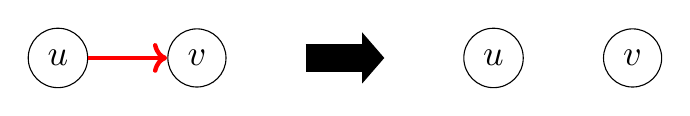
\begin{tikzpicture}[scale=1.3, node/.style={draw,circle,scale=1.3}]
            \node[node] (u1) {$u$};
            \node[node, right = of u1] (v1) {$v$};
            \coordinate[right = of v1] (a);
            \coordinate[right = of a] (b);
            \node[node, right = of b] (u2) {$u$};
            \node[node, right = of u2] (v2) {$v$};
    
            \draw[->, ultra thick, red] (u1) -- (v1);
            \draw[-{Triangle[width=18pt,length=8pt]}, line width=10pt] (a) -- (b);
        \end{tikzpicture}
    \end{figure}

    \item \textit{RI} --- remoção de vértices de grau um, somando os custos no vértice adjacente;

    \begin{figure}[H]
        \centering
        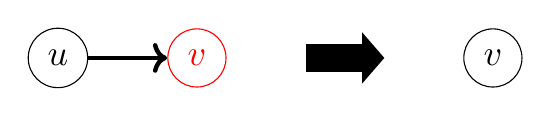
\begin{tikzpicture}[scale=1.3, node/.style={draw,circle,scale=1.3}]
            \node[node] (u1) {$u$};
            \node[node, right = of u1, red] (v1) {$v$};
            \coordinate[right = of v1] (a);
            \coordinate[right = of a] (b);
            
            \node[node, right = of b] (u2) {$v$};
    
            \draw[->, ultra thick, black] (u1) -- (v1);
            \draw[-{Triangle[width=18pt,length=8pt]}, line width=10pt] (a) -- (b);
        \end{tikzpicture}
    \end{figure}

    \item \textit{RII} --- remoção de vértices de grau dois, após os custos serem contabilizados na matriz de custos da nova aresta entre os dois vizinhos. Se necessário, a aresta é criada primeiro;

    \begin{figure}[H]
        \centering
        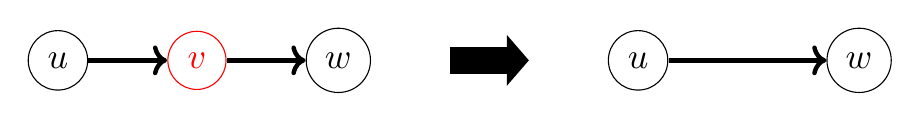
\begin{tikzpicture}[scale=1.3, node/.style={draw,circle,scale=1.3}]
            \node[node] (u1) {$u$};
            \node[node, right = of u1, red] (v1) {$v$};
            \node[node, right = of v1] (w1) {$w$};
            \draw[->, ultra thick, black] (u1) -- (v1);
            \draw[->, ultra thick, black] (v1) -- (w1);
            
            \coordinate[right = of w1] (a);
            \coordinate[right = of a] (b);

            \node[node, right = of b] (u2) {$u$};
            \coordinate[right = of u2] (c);
            \node[node, right = of c] (w2) {$w$};
            \draw[->, ultra thick, black] (u2) -- (w2);
            
            \draw[-{Triangle[width=18pt,length=8pt]}, line width=10pt] (a) -- (b);
        \end{tikzpicture}
    \end{figure}

    \item \textit{RN} --- remoção de vértices de grau três ou maior. Dado um vértice $u$, é escolhido um mínimo local e os custos de $u$ são distribuídos entre seus vizinhos. Em seguida, $u$ é removido e as arestas são removidas usando \textit{RE}.

    \begin{figure}[H]
        \centering
        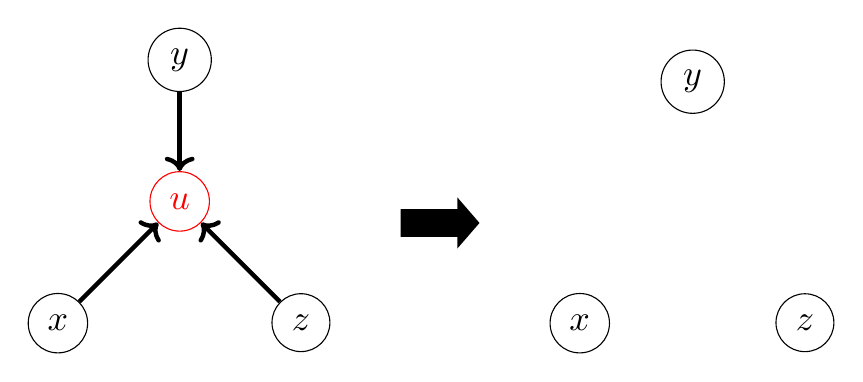
\begin{tikzpicture}[scale=1.3, node/.style={draw,circle,scale=1.3}]
            \node[node, red] (u) {$u$};
            \node[node, above = of u] (y1) {$y$};
            \node[node, below left = of u] (x1) {$x$};
            \node[node, below right = of u] (z1) {$z$};
            \draw[->, ultra thick, black] (x1) -- (u);
            \draw[->, ultra thick, black] (y1) -- (u);
            \draw[->, ultra thick, black] (z1) -- (u);
            
            \coordinate[above right = of z1] (a);
            \coordinate[right = of a] (b);
            \node[node, below right = of b] (x2) {$x$};
            \node[node, above right = of x2, white] (u2) {};

            \node[node, above = of u2] (y2) {$y$};
            \node[node, below right = of u2] (z2) {$z$};
            
            \draw[-{Triangle[width=18pt,length=8pt]}, line width=10pt] (a) -- (b);
        \end{tikzpicture}
    \end{figure}
\end{enumerate}

As reduções \textit{RE}, \textit{RI}, e \textit{RII} produzem subdivisões da instância original de igual custo mínimo, permitindo estender a seleção dos problemas menores para o problema original sem comprometer a qualidade da solução. Se o grafo inteiro puder ser reduzido dessa maneira, então é possível encontrar uma solução ótima para dada instância do problema. Se \textit{RN} for aplicada, no entanto, as subpartes produzidas perdem a precisão de representação do problema e a solução final obtida torna-se quase-ótima, onde a proximidade de uma hipotética solução ótima é garantida através da heurística de escolha do mínimo local como alternativa.

Hames e Scholz \cite{hames:06} propuseram, em 2006, uma heurística alternativa para a redução \textit{RN} que elimina a escolha de uma alternativa na etapa de redução, efetivamente a postergando para a fase de retropropagação das soluções. Além disso, eles intrudoziram um abordagem \textit{branch-and-bound} que consiste em utilizar de um limiar para dividir as possíveis combinações de escolhas, de tal modo que as combinações que certamente não são ótimas são descartadas e nunca são avaliadas pelo alocador. Essas heurísticas garantem resolução em tempo linear, e as reduções tornam a alocação via PBQP especialmente poderosa em instâncias que produzem grafos de interferência esparsos, pois permitem a alocação de maneira trivial.

\chapter{Minimização de \textit{Spill Code}}

Mesmo com a utilização de algoritmos refinados de alocação, em vários casos a introdução de \textit{spill code} no código resultante é factualmente inevitável. Sendo assim, um bom alocador deve produzir uma alocação visando minimizar o tráfego de dados entre a memória principal e o processador, devido ao grande \textit{overhead} provocado pela execução de instruções de acesso à memória. Essas operações são responsáveis pela maior parte do gasto energético em sistemas computacionais \cite{verma:06}, e a alocação de registradores pode impactar o tempo de execução de um programa em até 250\% \cite{pereira:08}.

Dentre os problemas enfrentados pelos desenvolvedores de compiladores, há a notável tarefa de se decidir qual registrador virtual será enviado para a memória. A escolha deve ser tomada de modo a reduzir a pressão de registradores nos pontos problemáticos do código, preferencialmente tornando-o inteiramente alocável e resolvendo o problema com o \textit{spill} de uma única variável. No entanto, a escolha de uma variável frequentemente acessada, que está dentro de um laço de repetição ou é usada como controle, pode acidentalmente produzir muito mais acessos à memória no programa \cite{chaitin:82, bernstein:89}.

Além disso, há espaço para diferentes análises na tarefa de se estimar custos de \textit{spill}. Diferentes métodos de se definir o custo das operações de acesso à memória e calcular o custo associado à escolha de cada variável são possíveis, e podem produzir resultados diferentes considerando a especificidade arquitetura-alvo. Sendo assim, os desenvolvedores de compiladores dependem de experimentação e "tentativa e erro" para ajustar suas heurísticas de alocação \cite{amarasinghe:03}.

\section{Heurísticas de Chaitin}

A proposta inicial do primeiro alocador via coloração de grafos, feita por Chaitin \textit{et al.} em 1981, não continha heurísticas significativas para otimizar a introdução de \textit{spill code}. Inicialmente, a prioridade de escolha para a realização de \textit{spill} era dada às variáveis denominadas \textit{pass-through} --- isto é, que estão vivas na entrada dos blocos básicos e não são usadas nem redefinidas posteriormente. Instruções de \texttt{store} eram inseridas após toda redefinição do \textit{live range} escolhido, e os \texttt{loads} eram necessários antes de qualquer uso \cite{chaitin:81}.

Sendo assim, em um trabalho posterior de 1982, Chaitin formalizou heurísticas para a tomada de decisões de \textit{spill} que almejavam reduzir a quantidade de acessos a memória em tempo de execução \cite{chaitin:82}. O custo de \textit{spill} de um registrador virtual é definido como o aumento no tempo de execução caso ele resida em memória, que corresponde ao número de pontos de definição mais o número de usos do valor. Por suas vezes, as definições e usos são ponderados levando em conta suas frequências estimadas de execução.

O custo de \textit{spill} associado a um \textit{live range} $v$ no alocador de Chaitin é dado pela fórmula \ref{chaitin-custo}. Nela, $i \in I$ é uma instrução contida na representação intermediária do programa, que manipula $v$ através de um uso ou uma redefinição, representados respectivamente pelos predicados $\textit{use}_v(i)$ e $\textit{def}_v(i)$. A função $\textit{profundidade} (i)$ expressa o nível de aninhamento de $i$ dentro de laços de repetição. 

\begin{equation}
    \textit{custo}(v) = \sum_{\mathclap{\substack{i \in I\\\textit{use}_v(i) \lor \textit{def}_v(i)}}} 10 ^ {\textit{profundidade}(i)}
    \label{chaitin-custo}
\end{equation}

Os custos são computados quando, durante a etapa de \textit{simplify}, não são encontrados mais vértices aptos a serem removidos do grafo de interferência e o algoritmo trava. Em seguida, o alocador define as prioridades para a escolha de qual variável sofrerá \textit{spill} utilizando a fórmula \ref{chaitin-prioridade}. Para cada \textit{live range}, o custo é dividido pelo grau do vértice correspondente no grafo e o vértice com menor valor ponderado é escolhido para sofrer \textit{spill} em todo o código \cite{bernstein:89}.

\begin{equation}
    h(v) = \frac{\textit{custo}(v)}{\textit{grau}(v)}
    \label{chaitin-prioridade}
\end{equation}

Chaitin \cite{chaitin:82} ainda introduziu o conceito de proximidade entre instruções: duas instruções são ditas próximas se nenhum \textit{live range} for eliminado entre elas e, consequentemente, nenhum registrador for liberado para alocação nesse intervalo. Esse princípio fundamenta um conjunto de três diretrizes que buscam evitar a inserção de \textit{reloads} desnecessários no código. São elas:
\begin{enumerate}
    \item Se uma definição e um uso são próximos, não é necessário adicionar um \texttt{load} antes do uso. Isso ocorre porque, como não foram disponibilizados novos registradores entre as instruções, o registrador da segunda instrução está disponível para a primeira. Sendo assim, é possível alocar o mesmo registrador para as duas utilizações;
    \item Se duas instruções de uso são próximas, é necessário introduzir um \texttt{load} somente antes do primeiro uso. De maneira análoga à diretriz anterior, o mesmo registrador pode ser reaproveitado na segunda instrução;
    \item Se a primeira definição e o último uso de um \textit{live range} são próximos, então o custo de \textit{spill} do registrador virtual é considerado infinito. Como nenhum registrador é liberado, enviar a variável para memória não tornará o programa colorível.
\end{enumerate}
    
\section{Heurísticas de Bernstein}

Em um trabalho de 1989, Bernstein \textit{et al.} \cite{bernstein:89} pontuaram uma série de problemas com o alocador de Chaitin. Em primeiro lugar, a heurística empregada na decisão de \textit{spill} pode não ser a mais eficiente em todas as instâncias de alocação. Além disso, o alocador de Chaitin insere instruções \texttt{store}/\texttt{load} desnecessariamente em todos os pontos do antigo \textit{live range}, sendo que elas podem somente ser necessárias em pontos de grande pressão de registradores. 

Sendo assim, o trabalho trouxe algumas técnicas e novas heurísticas visando expandir as contribuições de Chaitin. Essas melhorias se mostraram capazes de reduzir a quantidade de código \textit{spill}, na média, em 6\% e 12\%, chegando até 30\% em alguns casos.

\subsection{\textit{Best-of-three}}

Bernstein \textit{et al.} notaram que, a respeito da heurística de decisão de \textit{spill}, não se pode fazer uma afirmação absoluta sobre o desempenho de uma função heurística simples em relação a outra para todos os programas. Ao contrário, diferentes instâncias de problemas de alocação podem exigir estratégias distintas para a obtenção de melhores resultados. Eles propuseram comparar o desempenho médio de diferentes fórmulas, mantendo em mãos um seleto número funções heurísticas que vislumbrem as diferentes causas da pressão de registradores, e escolhendo a melhor delas para tomar as decisões de \textit{spill}.

A heurística $h_1$ (\ref{bernstein-1}) tem em vista a estratégia original de Chaitin, que consiste em escolher um vértice com baixo custo e alto grau. Realizar \textit{spill} de uma variável com alto grau reduz o grau de muitos outros vértices no grafo de interferência, tornando mais provável que outros vértices se tornem desobstruídos.

\begin{equation}
    h_1(v) = \frac{\textit{custo}(v)}{\textit{grau}(v)^2}
    \label{bernstein-1}
\end{equation}

Alternativamente, a abordagem escolhida pode ser a de se fazer \textit{spill} do registrador virtual que exerça a maior pressão de registradores sobre o código. Sendo assim, é introduzido o conceito de área de uma variável, computado através da fórmula:
\begin{equation}
    \textit{área}(v) = \sum_{\mathclap{\substack{i \in I\\v\text{ vivo em }i}}} 5 ^ {\textit{profundidade}(i)} \textit{largura}(i)
    \label{bernstein-area}
\end{equation}
onde $\textit{largura}(i)$ é o número de variáveis vivas no momento de execução da instrução $i$. De maneira intuitiva, $\textit{área}(v)$ expressa o impacto de $v$ para a pressão de registradores global. A escolha de uma variável com alta área causa uma redução considerável na pressão em todo o programa, e facilita a coloração. As heurísticas seguintes $h_2$ e $h_3$ (\ref{bernstein-2_3}) se fundamentam nesse princípio.

\begin{subequations}
    \begin{equation}
        h_2(v) = \frac{\textit{custo}(v)}
                      {\textit{área}(v)\textit{grau}(v)}
        \label{bernstein-2}
    \end{equation}
    \begin{equation}
        h_3(v) = \frac{\textit{custo}(v)}
                      {\textit{área}(v)\textit{grau}(v)^2}
        \label{bernstein-3}
    \end{equation}
    \label{bernstein-2_3}
\end{subequations}

O algoritmo proposto por Bernstein \textit{et al.} efetua efetua a coloração do grafo de interferência múltiplas vezes, para cada heurística $h_i$ disponível. O resultado final escolhido é o da heurística que produza o menor custo total de \textit{spill}. Essa técnica, apelidada de "\textit{best-of-three}", superou as abordagens anteriores consideravelmente, sob penalidade de um tempo de compilação ligeiramente maior.

\subsection{\textit{Coloração gulosa}}

Além disso, foram propostas heurísticas de coloração que se baseiam em adotar uma estratégia local para cada região do programa. É sabido que o grafo de interferência pode conter diversos subgrafos com diferentes características, sendo que alguns deles podem ser coloridos em tempo polinomial \cite{golumbic:04, dagan:88}. Dessa maneira, diferentes formas de coloração podem ser adotadas em diferentes porções do código, e os resultados combinados para compor a alocação final.

O algoritmo de coloração de por Bernstein \textit{et al.} realiza a etapa de \textit{simplify} removendo sempre o vértice apto de maior grau. Logo, na etapa de \textit{select}, os registradores são alocados em ordem crescente de grau para cada \textit{live range}. Ademais, após a $k$-colorabilidade do grafo de interferência ter sido assegurada, um critério secundário pode usado para colori-lo com, geralmente, menos cores do que em uma atribuição aleatória. Em certas situações, isso pode melhorar o código resultante, como:

\begin{enumerate}
    \item A alocação produziu \textit{spills} a mais, e torna-se possível colorir o grafo com menos do que $k$ cores. Nesse caso, as $k - n$ decisões de \textit{spill} mais custosas da iteração anterior podem ser desfeitas;
    \item Pequenos procedimentos chamados frequentemente, onde uma utilização de registradores econômica pode reduzir o \textit{overhead} das chamadas;
    \item Expansões \textit{inline} de funções, onde a decisão de expandir ou não é influenciada pela quantidade de registradores utilizados na sub-rotina.
\end{enumerate}

\subsection{\textit{Cleaning}}

Além do mais, Bernstein \textit{et al.} resolveram o problema da inserção desnecessária de instruões \texttt{store}/\texttt{load} através da técnica denominada pelos autores como "\textit{cleaning}", ou limpeza. Esse método consiste em, quando uma variável for enviada para a memória, inserir somente uma instrução \texttt{store} e um \texttt{load} por bloco básico. Ao examinar um bloco em busca de valores que sofreram \textit{spill}, os acessos à memória são introduzidos apenas no primeiro uso ou definição do \textit{live range}. Em seguida, a variável é renomeada em cada bloco básico em que é usada, fragmentando o tempo de vida original.

Os autores notaram que o \textit{cleaning} é bem sucedido em reduzir o número total de instruções de acesso à memória, especialmente nas primeiras duas iterações de coloração/\textit{spill}, e quando nenhuma restrição é imposta à profundidade dos blocos básicos nos quais a limpeza é realizada ou aos registradores para os quais a limpeza é aplicada.

\begin{algorithm}
    \caption{Algoritmo de coloração utilizando \textit{best-of-three}. Extraído de Bernstein \textit{et al.} \cite{bernstein:89}}.
    \begin{algorithmic}
        \Procedure{ColorAndSpill}{}
            \ForAll{heurística $h_i$}
                \While{$G$ não é vazio}{}
                    \If{existe um $v$ tal que $\textit{grau}(v) < |R|$}
                        \State escolha o $v$ com maior grau (tal que $\textit{grau}(v) < |R|$)
                        \State $G \gets G - \{v\}$
                    \Else
                        \State escolha um $v$ com $\textit{min }h_i(v)$
                        \State $S_i \gets S_i \cup {v}$
                        \State $G \gets G - \{v\}$
                    \EndIf
                \EndWhile
            \EndFor
        \EndProcedure
    \end{algorithmic}
\end{algorithm}

\section{\textit{Spilling} por Região de Interferência}

Em um trabalho de 1997, Bergner \textit{et al.} \cite{bergner:97} pontuou que as heurísticas prévias ainda produziam \textit{spill} code desnecessariamente, pois as instruções de acesso à memória eram inseridas ao longo de todo o tempo de vida que era escolhido para \textit{spill}. Em resposta a esse problema, Bergner \textit{et al.} introduziu o conceito de \textit{spilling} por região de interferência, que consistia em limitar as alterações no código somente às regiões de sobreposição entre os \textit{live ranges}, nos pontos de alta pressão de registradores.

Nessa abordagem, uma região de interferência entre dois registradores virtuais é dita como a porção do programa onde ambos estão vivos simultaneamente, e elas são diretamente representadas no grafo de interferência na forma das arestas. Em adição às técnicas de minimização de \textit{spill code} propostas por Chaitin \cite{chaitin:81}, Bernstein \cite{bernstein:89} e Briggs \cite{briggs2:92}, o alocador de Bergner limita a introdução de \textit{reloads} somente aos usos da variável dentro da região de interferência. No caso em que o \textit{live range} é utilizado novamente após a região de interferência, deve-se introduzir um \textit{reload} adicional para recarregar o valor de volta para um registrador físico.

Para escolher quais regiões de interferência sofrerão \textit{spill}, a estratégia desenvolvida por Bergner é aplicada durante a etapa de \textit{select} de um alocador ao estilo de Briggs, durante a reintrodução dos vértices no grafo e concomitante alocação de cores. Ao se tentar reintroduzir um vértice $v$ candidato a \textit{spill} --- o que não será inteiramente possível devido ao número de interferências de $v$, suas arestas são agrupadas em conjuntos, cada conjunto contendo as arestas que se conectam a vértices de uma mesma cor. O alocador deve então tentar colorir $v$, não inserindo no grafo as arestas do conjunto cuja cor já está atribuída a algum dos seus vizinhos. 

O custo de se fazer \textit{spill} de $v$ em cada região de interferência é calculado levando em conta a quantidade estimada de instruções \texttt{store}/\texttt{load} que serão introduzidas no código, e a cor selecionada para o vértice candidato deve ser a que minimize o total desse custo. Uma vez que a cor é definida, as regiões de interferência cujas arestas correspondentes não puderam ser inseridas no grafo são escolhidas para sofrerem \textit{spill}. As figuras \ref{bergner-3} e \ref{bergner-4} demonstram esse processo, onde o vértice candidato $A$ recebe a mesma cor de $C$, impedindo que a aresta $AC$ seja introduzida no grafo. Ela é então descartada, e $A$ sofrerá \textit{spill} na região de interferência entre $A$ e $C$.

A estratégia introduzida no trabalho Bergner \textit{et al.} mostrou grandes taxas de sucesso em experimentos, conquistando uma redução média de 33,6\% no número de instruções de acesso a memória executadas dinamicamente, atingindo a faixa de 75\% em alguns casos \cite{bergner:97}. Essa técnica superou de longe as heurísticas anteriores, e representou um avanço significativo na minimização de \textit{spill code}. 

\begin{figure}[h]
    \centering
    \begin{subfigure}{0.45\textwidth}
        \centering
        \begin{lstlisting}
    A = input();
    B = A + 1;
    if (A) {
        C = A + 2;
        B = A + C;
        if (C) {
            B = B + C;
            C = B + C;
        }
        A = B + C;
    }
    D = A + B;
        \end{lstlisting}
        \caption{Exemplo de programa em pseudocódigo.}
        \label{bergner-1}
    \end{subfigure}
    \begin{subfigure}{0.45\textwidth}
        \centering
        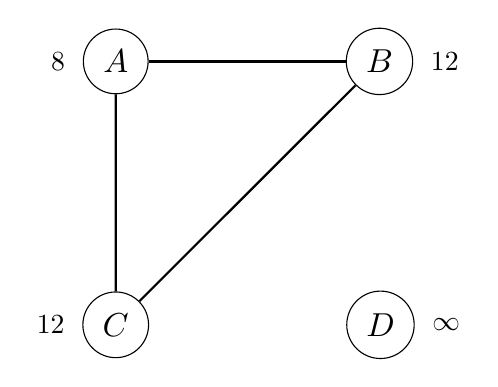
\begin{tikzpicture}[scale=2, node/.style={draw,circle, scale=1.2}]
            \node[node] (A) {$A$};
            \node[left = 1mm of A] {$8$};
            \node[node, right = 25mm of A] (B) {$B$};
            \node[right = 1mm of B] {$12$};
            \node[node, below = 25mm of A] (C) {$C$};
            \node[left = 1mm of C] {$12$};
            \node[node, right = 25mm of C] (D) {$D$};
            \node[right = 1mm of D] {$\infty$};

            \draw[black, thick] (A) -- (B);
            \draw[black, thick] (A) -- (C);
            \draw[black, thick] (C) -- (B);
        \end{tikzpicture}
        \caption{Grafo de interferência correspondente, com os custos de \textit{spill} indicados.}
        \label{bergner-2}
    \end{subfigure}
    \caption{Exemplo extraído de Bergner \textit{et al.} \cite{bergner:97}.}
\end{figure}

\begin{figure}[h]
    \centering
    \begin{subfigure}{0.45\textwidth}
        \centering
        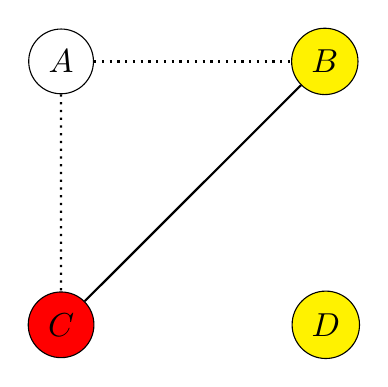
\begin{tikzpicture}[scale=2, node/.style={draw,circle, scale=1.2}]
            \node[node] (A) {$A$};
            \node[node, right = 25mm of A, fill=yellow] (B) {$B$};
            \node[node, below = 25mm of A, fill=red] (C) {$C$};
            \node[node, right = 25mm of C, fill=yellow] (D) {$D$};

            \draw[black, thick, dotted] (A) -- (B);
            \draw[black, thick, dotted] (A) -- (C);
            \draw[black, thick] (C) -- (B);
        \end{tikzpicture}
        \caption{Tentativa de coloração com duas cores. Nesse caso, $A$ torna-se candidato a \textit{spill}.}
        \label{bergner-3}
    \end{subfigure}
    \begin{subfigure}{0.45\textwidth}
        \centering
        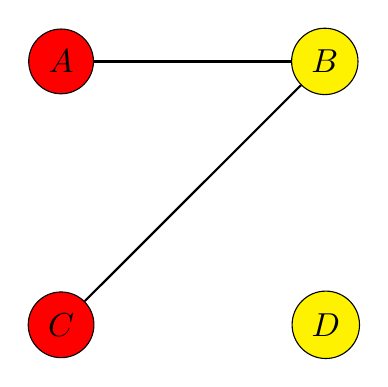
\begin{tikzpicture}[scale=2, node/.style={draw,circle, scale=1.2}]
            \node[node, fill=red] (A) {$A$};
            \node[node, right = 25mm of A, fill=yellow] (B) {$B$};
            \node[node, below = 25mm of A, fill=red] (C) {$C$};
            \node[node, right = 25mm of C, fill=yellow] (D) {$D$};

            \draw[black, thick] (A) -- (B);
            \draw[black, thick] (C) -- (B);
        \end{tikzpicture}
        \caption{$A$ recebe uma cor, e a região de interferência $AC$ é escolhida para \textit{spill}.}
        \label{bergner-4}
    \end{subfigure}
    \caption{Coloração do exemplo da figura \ref{bergner-2}, considerando a estratégia de \textit{spilling} por região de interferência. Adaptado de Bergner \textit{et al.} \cite{bergner:97}.}
\end{figure}

\begin{figure}
    \centering
    \begin{subfigure}{0.45\textwidth}
        \centering
        \begin{lstlisting}[mathescape=true]
    A = input();
    store A;
    B = A + 1;
    if (A) {
        load $A_1$;
        C = $A_1$ + 2;
        B = $A_1$ + C;
        if (C) {
            B = B + C;
            C = B + C;
        }
        $A_2$ = B + C;
        store $A_2$;
    }
    load $A_3$;
    D = A + B;
        \end{lstlisting}
        \caption{Código resultante ao se fazer \textit{spill} de $A$ em todo o programa.}
        \label{bergner-5}
    \end{subfigure}
    \begin{subfigure}{0.45\textwidth}
        \centering
        \begin{lstlisting}[mathescape=true]
    A = input();
    store A;
    B = A + 1;
    if (A) {
        load $A_1$;
        C = $A_1$ + 2;
        B = $A_1$ + C;
        if (C) {
            B = B + C;
            C = B + C;
        }
        A = B + C;
        
    }
    
    D = A + B;
        \end{lstlisting}
        \caption{Código resultante após o \textit{spill} somente na região de interferência $AC$.}
        \label{bergner-6}
    \end{subfigure}
    \caption{Caption}
\end{figure}

\section{Rematerialização}

Em seu trabalho de 1982, Chaitin \textit{et al.} \cite{chaitin:82} já haviam demonstrado que é preferível inserir instruções para recalcular certos valores ao invés de armazená-los em memória, devido ao custo mais baixo de fazê-lo. Essa técnica foi denominada "\textit{rematerialization}", ou rematerialização, e representa uma alternativa à geração de \textit{spill code} em situações onde a pressão de registradores ultrapassa o número de registradores físicos disponíveis. Posteriormente, Briggs \textit{et al.} \cite{briggs2:92} refinaram essa técnica, introduzindo novos conceitos e propondo uma metodologia que permite uma otimização mais profunda.

Chaitin \textit{et al.} mostraram que certos valores podem ser recalculados com uma única instrução adicional, caso os operandos necessários estejam sempre disponíveis. Eles denominaram esses casos excepcionais como valores \textit{"never-killed"}, e argumentaram que é mais barato recomputar tais valores do que armazená-los e constantemente acessar a memória para recuperá-los. Na prática, boas oportunidades para a rematerialização incluem \texttt{loads} imediatos de constantes e o cálculo de endereços de memória, com ou sem \textit{offset}. Entretanto, o alocador de Chaitin só pode rematerializar \textit{live ranges} que assumem um único valor ao longo de toda sua extensão, não sendo capaz de lidar com casos mais complexos.

Sendo assim, em 1992 Briggs \textit{et al.} expandiram a técnica de Chaitin para tratar \textit{live ranges} multivalorados. Sua abordagem consistia em dividir os tempos de vida para cada valor que assumem ao longo da execução de um programa, efetivamente convertendo a representação intermediária para a forma SSA (\textit{static single-assignment}). Na forma SSA, cada variável é definida uma única vez antes de ser obrigatoriamente usada, e por isso possui apenas um valor ao longo do seu tempo de vida. No processo de conversão para a forma SSA, os \textit{live ranges} dão origem vários tempos de vida menores definidos uma única vez, a partir de um valor simples ou uma função-$\phi$ --- artifício que representa a utilização de um dentre múltiplos valores possíveis em tempo de execução.

\begin{figure}[h]
    \centering
    \begin{subfigure}%[align=c]
    {0.45\textwidth}
        \centering
        
        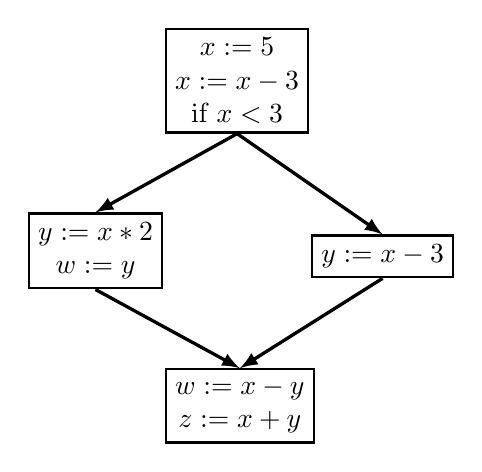
\begin{tikzpicture}[CFG/.style={rectangle, draw=black!100, fill=white!100, thick, minimum size=5mm, align=center}]

            \node[CFG] (B0) {$x:=5$\\
                             $x:=x-3$\\
                             if $x<3$};
    
            \node[CFG, below right = 12.8mm and 0.2mm of B0] (B1) 
                {$y:=x-3$};
            \node[CFG, below left = 10mm and 0.2mm of B0] (B2) 
                {$y:=x * 2$\\
                 $w:=y$};
            \node[CFG, below right = 10mm and 0.2mm of B2] (B3) 
                {$w:=x-y$\\
                 $z:=x+y$};

            \draw[-latex, black, very thick] (B0.south) -- (B1.north) {};
            \draw[-latex, black, very thick] (B0.south) -- (B2.north) {};
            \draw[-latex, black, very thick] (B1.south) -- (B3.north) {};
            \draw[-latex, black, very thick] (B2.south) -- (B3.north) {};
        \end{tikzpicture}
        \caption{Grafo de controle de fluxo na forma tradicional.}
        \label{ssa-1}
    \end{subfigure}
    \begin{subfigure}%[align=c]
    {0.45\textwidth}
        \centering
        
        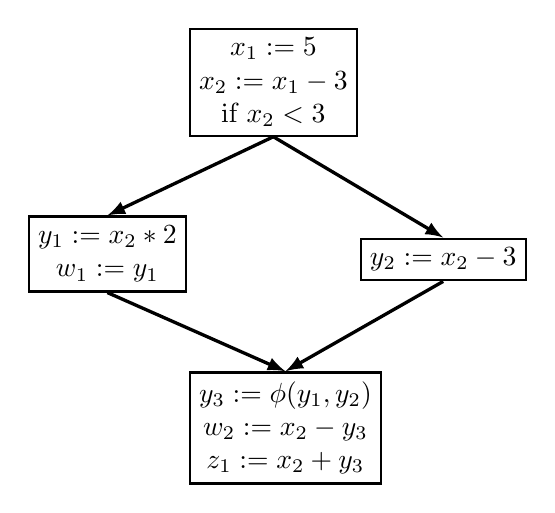
\begin{tikzpicture}[CFG/.style={rectangle, draw=black!100, fill=white!100, thick, minimum size=5mm, align=center}]

            \node[CFG] (B0) {$x_1:=5$\\
                             $x_2:=x_1-3$\\
                             if $x_2<3$};
    
            \node[CFG, below right = 12.8mm and 0.2mm of B0] (B1) 
                {$y_2:=x_2-3$};
            \node[CFG, below left = 10mm and 0.2mm of B0] (B2) 
                {$y_1:=x_2 * 2$\\
                 $w_1:=y_1$};
            \node[CFG, below right = 10mm and 0.2mm of B2] (B3) 
                {$y_3:=\phi(y_1,y_2)$\\
                 $w_2:=x_2-y_3$\\
                 $z_1:=x_2+y_3$};

            \draw[-latex, black, very thick] (B0.south) -- (B1.north) {};
            \draw[-latex, black, very thick] (B0.south) -- (B2.north) {};
            \draw[-latex, black, very thick] (B1.south) -- (B3.north) {};
            \draw[-latex, black, very thick] (B2.south) -- (B3.north) {};
        \end{tikzpicture}
        \caption{O mesmo grafo na forma SSA, onde $y_3$ pode receber o valor de $y_1$ ou $y_2$.}
        \label{ssa-2}
    \end{subfigure}
    \caption{Exemplo de código de três endereços na forma tradicional e forma SSA.}
\end{figure}

Em seguida, as instruções de definição dos valores são rotuladas como candidatas ou não à rematerialização. Para isso, Briggs \textit{et al.} empregaram um algoritmo semelhante ao \textit{constant propagation} de Wegman e Zadeck \cite{wegman:91}, para propagar as rotulações pelo grafo de controle de fluxo. Os rótulos consistem de:
\begin{enumerate}
    \item $\top$ --- significa que nenhuma informação é conhecida. Um valor definido por uma instrução de cópia ou uma função-$\phi$ recebem este rótulo de imediato;
    \item \textit{inst} --- valor definido por uma instrução adequada (\textit{never-killed}. Na implementação é um ponteiro para a própria instrução;
    \item $\bot$ --- valor que deve sofrer \textit{spill}. Valores inapropriados para a rematerialização recebem este rótulo de imediato.
\end{enumerate}

Além disso, quando o rótulo de uma variável é propagado para as instruções que a utilizam ocorre uma operação de encontro, denotada pelo símbolo $\sqcap$. Ela é definida como:
\begin{subequations}
    \begin{equation}
        x \sqcap \top = x
    \end{equation}
    \begin{equation}
        x \sqcap \bot = \bot
    \end{equation}
    \begin{equation}
        \textit{inst}_i \sqcap \textit{inst}_j = 
        \begin{cases}
            \textit{inst}_i, & \text{se } \textit{inst}_i = \textit{inst}_j \\
            \bot, & \text{se } \textit{inst}_i \ne \textit{inst}_j
        \end{cases}
    \end{equation}
\end{subequations}
onde $x$ é qualquer rótulo, e a comparação $\textit{inst}_i = \textit{inst}_j$ é realizada operando a operando. Os valores são todos inicializados como $\top$, e durante a propagação valores definidos por uma instrução de cópia terão seus rótulos reduzidos para \textit{inst} ou $\bot$. Valores definidos por funções-$\phi$ serão reduzidos para \textit{inst} se e somente se todos os valores o atingindo tiverem rótulos equivalentes; caso contrário, eles recebem $\bot$.

Concluída a propagação, os nós-$\phi$ devem ser removidos e os valores renomeados para que o programa executável seja produzido. Valores rotulados como \textit{never-killed} são rematerializados no código final e possíveis divisões desnecessárias dos \textit{live ranges}, remanescentes da forma SSA, são removidas através de processos presentes em um alocador estilo Briggs \cite{briggs:92}, como coalescimento e coloração com a mesma cor de variáveis unidas por cópia.

O algoritmo de Briggs \textit{et al.} foi testado em 70 benchmarks, apresentando uma redução considerável de \textit{spill code} em 28 dos casos, com melhorias que ultrapassaram os 20\%. Os autores também observaram uma redução nas instruções de \texttt{store}, \texttt{load} e de cópia, o que indica que as heurísticas de remoção de divisões desnecessárias são adequadas \cite{briggs2:92}.

\section{Coloração de grafos hierárquica}

Em 1991, Callahan e Koblenz \cite{callahan:91} descreveram uma técnica de alocação de registradores que emprega heurística hierárquica de coloração de grafos, onde o programa é particionado em uma série de porções que constituem uma estrutura de árvore e que refletem a estrutura de controle do código. Então, para cada porção é realizada a coloração de grafos de maneira local, resultando numa alocação sensível aos padrões de utilização das variáveis em cada região do programa.

O princípio da abordagem de Callahan e Koblenz consiste em representar o fluxo de repetição e ramificação nos blocos básicos na forma de \textit{"tiles"} que na prática constituem subárvores. Sendo o grafo de controle de fluxo (CFG) representado pela tupla $G = (B, E, \textit{start}, \textit{stop})$, onde $B$ é o conjunto dos blocos básicos, $E$ é o conjunto de arestas entre os blocos e $\textit{start}, \textit{stop} \in B$ representam respectivamente os pontos de início e fim do fluxo de execução, é definido uma árvore hierárquica $T$.

Cada nó $t \in T$ é um membro da família de subconjuntos de $B$ tal que $\textit{blocos}(t) = \{b_0, b_1, \dots, b_n\}$, onde $b \in B$ são os blocos básicos pertencentes a $t$, mas que não pertencem a nenhuma subárvore de $t$. Cada par de elementos em $t_1, t_2 \in T$ é ou disjunto, ou $t_1$ é subconjunto próprio de $t_2$ e não há nenhum outro $t$ tal que $t_1 \subset t \subset t_2$; nesse caso, dizemos que $t_1$ é nó-filho de $t_2$ e $t_2$ é nó-pai de $t_1$. Há também em todo programa uma raiz $t_0$ tal que $\textit{blocos}(t_0) = \{\textit{start}, \textit{stop}\}$. A adição de novos nós na árvore do programa ocorre nas ramificações criadas por estruturas condicionais e em laços de repetição, como exemplificado na figura \ref{arvore-programa}.

\begin{figure}[ht]
    \centering
    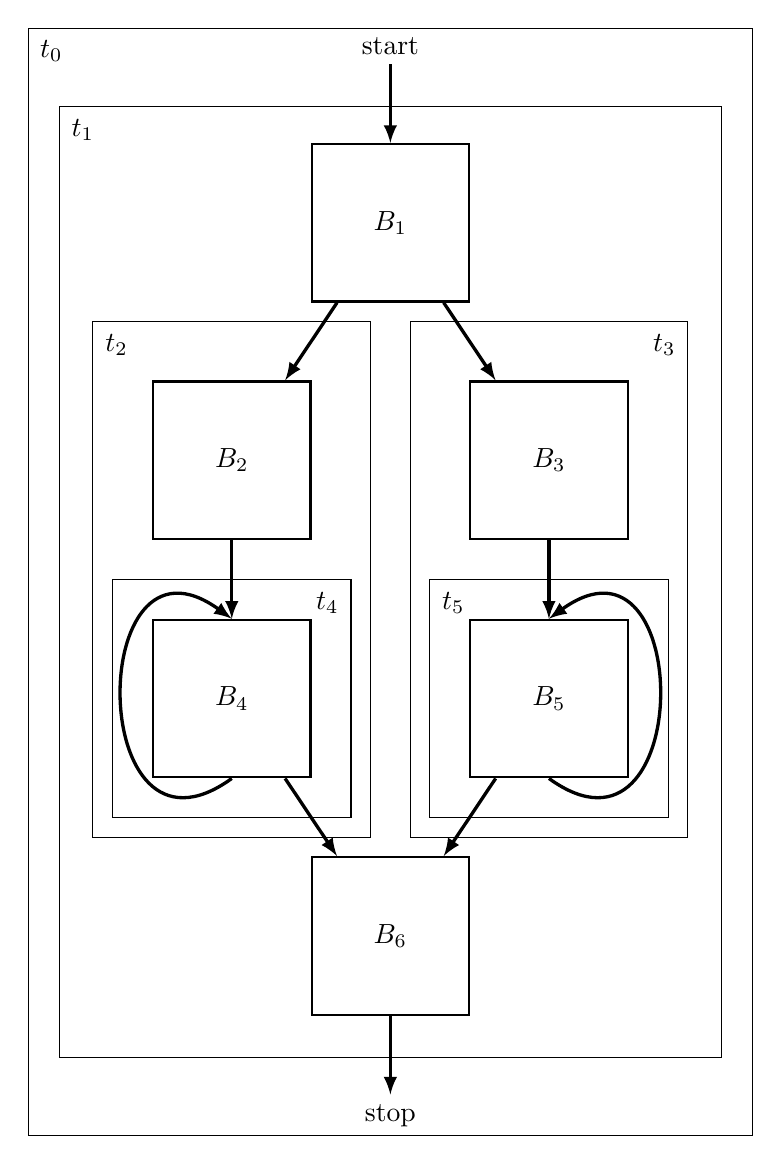
\begin{tikzpicture}[CFG/.style={rectangle, draw=black!100, fill=white!100, thick, minimum size=20mm, align=center}]
        \node (start) {start};
        \node[CFG, below = of start] (B1) {$B_1$};
        \coordinate[below = 20mm of B1] (C1);
        \node[CFG, left = of C1] (B2) {$B_2$};
        \node[CFG, right = of C1] (B3) {$B_3$};
        \node[CFG, below = of B2] (B4) {$B_4$};
        \node[CFG, below = of B3] (B5) {$B_5$};
        \coordinate[right = of B4] (C2);
        \node[CFG, below = 20mm of C2] (B6) {$B_6$};
        \node[below = of B6] (stop) {stop};

        \draw[-latex, very thick] (start) -- (B1);
        \draw[-latex, very thick] (B1) -- (B2);
        \draw[-latex, very thick] (B1) -- (B3);
        \draw[-latex, very thick] (B2) -- (B4);
        \draw[-latex, very thick] (B3) -- (B5);
        \draw[-latex, very thick] (B4) -- (B6);
        \draw[-latex, very thick] (B5) -- (B6);
        \draw[-latex, very thick] (B6) -- (stop);

        \coordinate[below left = 13.5mm and 8.5mm of B4] (E1);
        \coordinate[above left = 13.5mm and 8.5mm of B4] (E2);

        \coordinate[below right = 13.5mm and 8.5mm of B5] (E3);
        \coordinate[above right = 13.5mm and 8.5mm of B5] (E4);
        
        \draw[-latex, very thick] (B4.south) .. controls (E1) and (E2) .. (B4.north);
        \draw[-latex, very thick] (B5.south) .. controls (E3) and (E4) .. (B5.north);

        \coordinate[below left = of B4] (F1);
        \coordinate[below right = of B4] (F2);
        \coordinate[above left = of B4] (F3);
        \coordinate[above right = of B4] (F4);

        \draw ([xshift = 7mm] current bounding box.north east) -- ([xshift = -7mm] current bounding box.north west) -- ( current bounding box.south west) -- (current bounding box.south east) -- cycle;
        \node at ([xshift = 3mm, yshift = -3mm] current bounding box.north west) {$t_0$};

        \draw ([xshift = -4mm, yshift = -10mm] current bounding box.north east) -- ([xshift = 4mm, yshift = -10mm] current bounding box.north west) -- ([xshift = 4mm, yshift = 10mm] current bounding box.south west) -- ([xshift = -4mm, yshift = 10mm] current bounding box.south east) -- cycle;
        \node at ([xshift = 7mm, yshift = -13mm] current bounding box.north west) {$t_1$};

        \draw ([xshift = 7.5mm, yshift = 7.5mm] B2.north east) -- ([xshift = -7.5mm, yshift = 7.5mm] B2.north west) -- ([xshift = -7.5mm, yshift = -7.5mm] B4.south west) -- ([xshift = 7.5mm, yshift = -7.5mm] B4.south east) -- cycle;
        \node at ([xshift = -4.5mm, yshift = 4.5mm] B2.north west) {$t_2$};

        \draw ([xshift = 7.5mm, yshift = 7.5mm] B3.north east) -- ([xshift = -7.5mm, yshift = 7.5mm] B3.north west) -- ([xshift = -7.5mm, yshift = -7.5mm] B5.south west) -- ([xshift = 7.5mm, yshift = -7.5mm] B5.south east) -- cycle;
        \node at ([xshift = 4.5mm, yshift = 4.5mm] B3.north east) {$t_3$};

        \draw ([xshift = 5mm, yshift = 5mm] B4.north east) -- ([xshift = -5mm, yshift = 5mm] B4.north west) -- ([xshift = -5mm, yshift = -5mm] B4.south west) -- ([xshift = 5mm, yshift = -5mm] B4.south east) -- cycle;
        \node at ([xshift = 2mm, yshift = 2mm] B4.north east) {$t_4$};

        \draw ([xshift = 5mm, yshift = 5mm] B5.north east) -- ([xshift = -5mm, yshift = 5mm] B5.north west) -- ([xshift = -5mm, yshift = -5mm] B5.south west) -- ([xshift = 5mm, yshift = -5mm] B5.south east) -- cycle;
        \node at ([xshift = -2mm, yshift = 2mm] B5.north west) {$t_5$};
    \end{tikzpicture}
    \caption{Exemplo da árvore hierárquica de um programa.}
    \label{arvore-programa}
\end{figure}

Uma vez que a representação intermediária é organizada na forma da árvore hierárquica, a coloração de grafos é efetuada para cada nó de maneira recursiva em pós-ordem, ou \textit{"bottom-up"}. Para cada nó $t$, o grafo é montado contendo somente as variáveis cujo \textit{live range} é definido e usado inteiramente em $\textit{blocos}(t)$, que são denominadas variáveis locais, e a coloração é feita de maneira convencional seguindo um algoritmo ao estilo de Briggs \cite{briggs:89}. Para todos os fins, as variáveis globais a $t$ --- isto é, que são definidas em níveis superiores da árvore e estão vivas na entrada dos blocos básicos de um nó --- são ignoradas, pois serão tratadas na alocação de algum nó ancestral de $t$. Uma vez concluída a coloração, as variáveis recebem registradores físicos diretamente ou pseudoregistradores, que funcionam como alcunhas para grupos de registradores da arquitetura-alvo. 

Ao retornar para a chamada anterior da recursão, o algoritmo prossegue colorir o grafo do nó-pai $t_{pai}$ incluindo um conjunto de novas variáveis, cada uma delas sendo o coalescimento de todas as variáveis de $t$ que foram alocadas a um registrador distinto. Elas são denominadas "variáveis de resumo", e servem o propósito de indicar quais registradores já foram aproveitados na subárvore com raiz em $t$. Sendo assim, uma aresta é inserida no grafo de interferência de um nó se:
\begin{enumerate}
    \item Duas variáveis locais ao nó interferem em algum ponto de seus blocos;
    \item Uma variável global interfere com uma variável de resumo ou outra variável global;
    \item Uma variável está viva em uma subárvore de $t$ mas não consta nas variáveis de resumo vindas da subárvore;
    \item Uma variável de resumo conflita com outras variáveis de resumo da mesma subárvore.
\end{enumerate}

Uma vez que a raiz da árvore é colorida, a atribuição final de registradores  físicos ocorre de maneira \textit{"top-down"}, assim como a inserção de instruções de \textit{spill}. O \textit{spill code} é, de maneira geral, inserido nas entradas e saídas dos blocos básicos e consiste de instruções de acesso a memória para variáveis locais que sofreram \textit{spill} em um nó, instruções de cópia para variáveis que receberam registradores diferentes no nó pai e no nó filho, além de instruções \texttt{load} para recarregar valores que receberam um registrador no nó pai mas sofreram \textit{spill} no nó filho.

Para decidir quais \textit{live ranges} devem receber um registrador ou não é empregada uma heurística de decisão de \textit{spill} similar à de Chaitin \cite{chaitin:82}, com a adição de uma nova fórmula para o cálculo de custo desenvolvida por Callahan e Koblenz. Supondo custo unitário para as operações de acesso à memória, são apresentadas as fórmulas:
\begin{subequations}
    \begin{equation}
        \textit{peso\,local}_t(v) = \sum_{\mathclap{b \in \textit{blocos}(t)}} \textit{prob}(b) \textit{ref}_b(v)
    \end{equation}
    \begin{equation}
        \textit{transferência}_t(v) = \sum_{\mathclap{e \in \textit{arestas}(t)}} \textit{prob}(e) \textit{viva}_e(v)
    \end{equation}
    % \begin{equation}
    %     \textit{peso}_t(v) = \sum_{\mathclap{\substack{s\\s \text{ é nó filho de } t}}} (\textit{reg}_s(v) - \textit{mem}_s(v)) + \textit{peso\_local}_t(v)
    % \end{equation}
\end{subequations}
onde $\textit{peso\_local}_t$ corresponde ao custo de se manter um valor em registradores físicos levando em conta $\textit{blocos}(t)$, $\textit{transferência}_t$ é o custo de se inserir \textit{spill code} nas entradas e saídas dos blocos de $t$. As métricas $\textit{prob}(b)$ e $\textit{prob}(e)$ expressam respectivamente a probabilidade de um bloco e de uma aresta serem executados; $\textit{ref}_b(v)$ denota o número de referências a $v$ no bloco $b$ e $\textit{viva}_e(v)$ é uma função booleana que indica se $v$ está viva na aresta $e$.

A heurística de custo que fundamenta a decisão de qual variável deve sofrer \textit{spill} é dada pela função $\textit{peso}_t$, computada segundo as fórmulas:
\begin{subequations}
    \begin{equation}
        \textit{peso}_t(v) = \sum_{\mathclap{\substack{s\\s \text{ é nó-filho de } t}}} (\textit{reg}_s(v) - \textit{mem}_s(v)) + \textit{peso\,local}_t(v)
    \end{equation}
    \begin{equation}
        \textit{reg}_t(v) = \textit{reg?}_t(v)\textit{min}\{\textit{transferência}_t(v), \textit{peso}_t(v)\}
    \end{equation}
    \begin{equation}
        \textit{mem}_t(v) = \textit{mem?}_t(v)\textit{transferência}_t(v)
    \end{equation}
\end{subequations}
onde $\textit{reg?}_t(v)$ retorna $1$ se $v$ já tiver sido alocado a um registrador no nó $t$ e $0$ caso contrário, enquanto $\textit{mem?}_t(v)$ retorna $1$ se $v$ sofreu \textit{spill} em $t$ e $0$ caso contrário. A função $\textit{reg}_t(v)$ representa o prejuízo de se fazer \textit{spill} de $v$ no nó-pai de $t$, sendo que a variável foi alocada a um registrador em $t$, enquanto a função $\textit{mem}_t(v)$ representa o custo de se alocar $v$ a um registrador em um nó-pai sendo que $v$ sofreu \textit{spill} em $t$.

O alocador é capaz então de combinar as heurísticas de custo a uma análise da estrutura hierárquica do programa para minimizar a inserção de \textit{spill code}, analisando quando é proveitoso alocar uma variável para registrador ou enviá-la para memória. Por exemplo, pode ser preferível realizar \textit{spill} de uma variável $v$ definida em um nó $t$ que sofreu \textit{spill} em todas as subárvores abaixo de $t$, pois isso tornaria desnecessário todo o \textit{spill code} inserido nos nós descendentes de $t$ e a quantidade de instruções de acesso a memória seria potencialmente reduzida. Nesse caso, $\textit{peso}_t(v) < 0$ indicaria um desincentivo para se alocar um registrador para $v$, independente de sua coloribilidade.

O principal objetivo atingido por Callahan e Koblenz era o de se obter um método de alocação que tirasse proveito do paralelismo da máquina que executa o compilador. Eles observaram aproveitamento dos recursos de paralelismo ao realizar experimentos com um compilador de Fortran \cite{callahan:91}, confirmando as expectativas prévias da dupla.

\section{\textit{Live Range Splitting}}

Em 1998, Cooper \textit{et al.} \cite{cooper:98} introduziram um novo método heurístico para minimizar a inserção de código \textit{spill}, denominado \textit{live range splitting}. Cooper \textit{et al.} notaram que trabalhos anteriores já haviam proposto técnicas que realizavam a quebra de \textit{live ranges} em pedaços menores e demonstravam melhorias no \textit{spill code} produzido \cite{briggs:92, briggs2:92, chow:84}. No entanto, essas técnicas eram pouco ajustadas e não aproveitavam de maneira eficiente as oportunidades para dividir os \textit{live ranges} e reduzir a quantidade de acessos à memória por serem demasiado agressivas. Sendo assim, eles desenvolveram uma heurística mais precisa para efetuar a quebra dos tempos de vida em pontos estratégicos do programa e obter as melhorias desejadas.

A heurística de Cooper \textit{et al.} usa uma estratégia mais conservadora para efetuar a separação dos tempos de vida ao somente fazê-lo como alternativa à realização de \textit{spill} de uma variável. Dessa maneira, o alocador computaria o custo de se fazer \textit{spill} e compará-lo-ia ao custo de \textit{split} de uma variável candidata, escolhendo a opção menos dispendiosa. Por conseguinte, a separação de \textit{live ranges} ocorre somente em pontos de alta pressão de registradores, onde uma variável é quebrada ao redor de outra de modo a reduzir a pressão, e o \textit{overhead} causado pela criação de novos \textit{live ranges} desnecessários é evitado.

Chaitin \textit{et al.} \cite{chaitin:82} já haviam pontuado que a inserção de \textit{spill code} não elimina completamente as interferências de uma variável, mas apenas reduz a "área de contato" ao gerar \textit{live ranges} menores. Cooper \textit{et al.} notaram no entanto que se um \textit{live range} $v_1$ contém completamente um segundo \textit{live range} $v_2$, isto é, $v_1$ é vivo em todos os pontos da definição até o último uso de $v_2$, fazer \textit{spill} de $v_2$ não eliminará a interferência $v_1v_2$. Dessa forma, a única forma de eliminar a interferência para este caso seria efetuar \textit{spill} de $v_1$ ao redor do tempo de vida de $v_2$, efetivamente dividindo $v_1$ em duas partes, como exemplificado pela figura \ref{fig:splitting-1}.

\begin{figure}[ht]
    \centering
    \begin{subfigure}{0.45\textwidth}
        \centering
        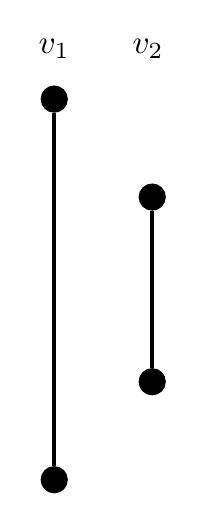
\begin{tikzpicture}[point/.style={circle, draw=black!100, fill=black!100, minimum size=2mm, align=center}]
            \node[point] (v_1_0) {};
            \node[above = 2mm of v_1_0, scale=1.2] (v_1_label) {$v_1$};
            \node[right = 5mm of v_1_label, scale=1.2] (v_2_label) {$v_2$};
            \node[point, below right = of v_1_0] (v_2_0) {};
            \node[point, below = 20mm of v_2_0] (v_2_1) {};
            \node[point, below left = of v_2_1] (v_1_1) {};
    
            \draw[-, ultra thick] (v_1_0) -- (v_1_1);
            \draw[-, ultra thick] (v_2_0) -- (v_2_1);
        \end{tikzpicture}
    \end{subfigure}
    \begin{subfigure}{0.45\textwidth}
        \centering
        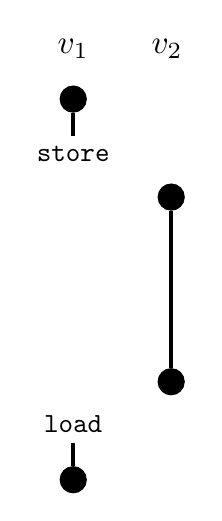
\begin{tikzpicture}[point/.style={circle, draw=black!100, fill=black!100, minimum size=2mm, align=center}]
            \node[point] (v_1_0) {};
            \node[above = 2mm of v_1_0, scale=1.2] (v_1_label) {$v_1$};
            \node[right = 5mm of v_1_label, scale=1.2] (v_2_label) {$v_2$};
            \node[point, below right = of v_1_0] (v_2_0) {};
            \node[below = 3mm of v_1_0] (store) {\texttt{store}};
            \node[point, below = 20mm of v_2_0] (v_2_1) {};
            \node[point, below left = of v_2_1] (v_1_1) {};
            \node[above = 3mm of v_1_1] (load) {\texttt{load}};
    
            \draw[-, ultra thick] (v_1_0) -- (store);
            \draw[-, ultra thick] (v_1_1) -- (load);
            \draw[-, ultra thick] (v_2_0) -- (v_2_1);
        \end{tikzpicture}
    \end{subfigure}
    \caption{Exemplo de \textit{splitting}. Nesse caso, $v_1$ é dividido ao redor de $v_2$, eliminando a interferência.}
    \label{fig:splitting-1}
\end{figure}

De modo a contemplar as relações de contenção entre os \textit{live ranges}, o \textit{live range splitting} requer a construção de um grafo direcionado $C$, denominado grafo de contenção. Os nós de $C$ representam as variáveis, enquanto uma aresta $e=(v_2,v_1)$ indica que $v_1$ estava vivo em uma definição ou uso de $v_2$.

\begin{figure}[ht]
    \centering

    \caption{lalala}
    \label{fig:splitting-2}
\end{figure}

\section{\textit{Outras Técnicas}}

\chapter{Aprendizado de Máquina}

\section{Paradigmas de Aprendizado}

\subsection{Aprendizado Supervisionado}

\subsection{Aprendizado Não-Supervisionado}

\section{Redes Neurais Artificiais}

\subsection{Aprendizado Profundo}

\chapter{A Infraestrutura LLVM}

\chapter{Trabalhos combinando Alocação de Registradores e Aprendizado de Máquina}

\chapter{Conclusão}

% ----------------------------------------------------------
% ELEMENTOS PÓS-TEXTUAIS
% ----------------------------------------------------------
\postextual


% ----------------------------------------------------------
% Referências bibliográficas
% ----------------------------------------------------------
\bibliography{abntex2-modelo-references}


% ----------------------------------------------------------
% Glossário
% ----------------------------------------------------------
%
% Consulte o manual da classe abntex2 para orientações sobre o glossário.
%
%\glossary

% ----------------------------------------------------------
% Apêndices
% ----------------------------------------------------------

% ---
% Apêndices (elemento opcional)
%
% São textos ou documentos elaborados pelo autor do trabalho a fim complementar
% a sua argumentação.
% ---
\begin{apendicesenv}

% Imprime uma página indicando o início dos apêndices
\partapendices

% ----------------------------------------------------------
\chapter{Quisque libero justo}
% ----------------------------------------------------------

\lipsum[50]

\end{apendicesenv}
% ---


% ----------------------------------------------------------
% Anexos (elemento opcional)
%
% São textos ou documentos, não elaborado pelo autor do trabalho que podem servir como
% ilustração, comprovação ou que contribua de forma relevante com o conteúdo já apresentado.
% ----------------------------------------------------------

% ---
% Inicia os anexos
% ---
\begin{anexosenv}

% Imprime uma página indicando o início dos anexos
\partanexos

% ---
\chapter{Morbi ultrices rutrum lorem.}
% ---
\lipsum[30]

\end{anexosenv}


% ----------------------------------------------------------
% Trabalhos publicados pelo autor
%
% Elemento obrigatório para as dissertações e teses do Programa
% de Pós-graduação em Ciência da Computação da UEL.
% (TCCs e monografias não precisam incluir essa seção)
% ----------------------------------------------------------
\chapter*{Trabalhos Publicados pelo Autor}
\addcontentsline{toc}{chapter}{Trabalhos Publicados pelo Autor}

\noindent
Trabalhos publicados pelo autor durante o programa.

% Elemento OBRIGATÓRIO somente para teses de doutorado e dissertações de mestrado no template DC/UEL).
% Listar publicações principais do trabalho (i.e., diretamente relacionados ao tema) e complementares, quando existirem.
% Listar em ordem decrescente de importância e/ou em ordem decrescente de ano de publicação.

\vspace{12pt}

\noindent
Publicações principais do trabalho.

\begin{enumerate}

\item Jose da silva, autor2 da silva, orientador da silva, \textbf{Título do artigo}, local onde foi
publicado, mês/ano, editora, número de página, isbn, etc. (Qualis CC 2017, xx)

\item Jose da silva, autor2 da silva, orientador da silva, \textbf{Título do artigo}, local onde foi
publicado, mês/ano, editora, número de página, isbn, etc. (Qualis CC 2017, xx)

\item Jose da silva, autor2 da silva, orientador da silva, \textbf{Título do artigo}, local onde foi
publicado, mês/ano, editora, número de página, isbn, etc. (Qualis CC 2017, xx)

\end{enumerate}

\noindent
Publicações complementares.

\begin{enumerate}

\item Jose da silva, autor2 da silva, orientador da silva, \textbf{Título do artigo}, local onde foi
publicado, mês/ano, editora, número de página, isbn, etc. (Qualis CC 2017, xx)

\item Jose da silva, autor2 da silva, orientador da silva, etc. \textbf{Título do artigo}, local onde foi
publicado, mês/ano, editora, número de página, isbn, (Qualis CC 2017, xx)

\end{enumerate}


%---------------------------------------------------------------------
% INDICE REMISSIVO (elemento opcional)
%---------------------------------------------------------------------
% Requer incluir instruções \index{...} no decorrer do texto, para marcar os termos a serem indexados

\printindex

\end{document}
